\chapter{Numerical Results}

\section{Rigid Body in Fluid Flow}

\subsection*{Compressible Fluid}

\subsection*{Incompressible Fluid}



\section{Parachute System Simulation}
With our spring-mass model and the numerical methods mentioned above, we can
simulate different types of parachute on \FronTierp platform.
\Fig{canopies} shows three types of parachute canopy after fully
inflated due to the interaction from the inflow air.
\begin{figure}[!ht]
\centering
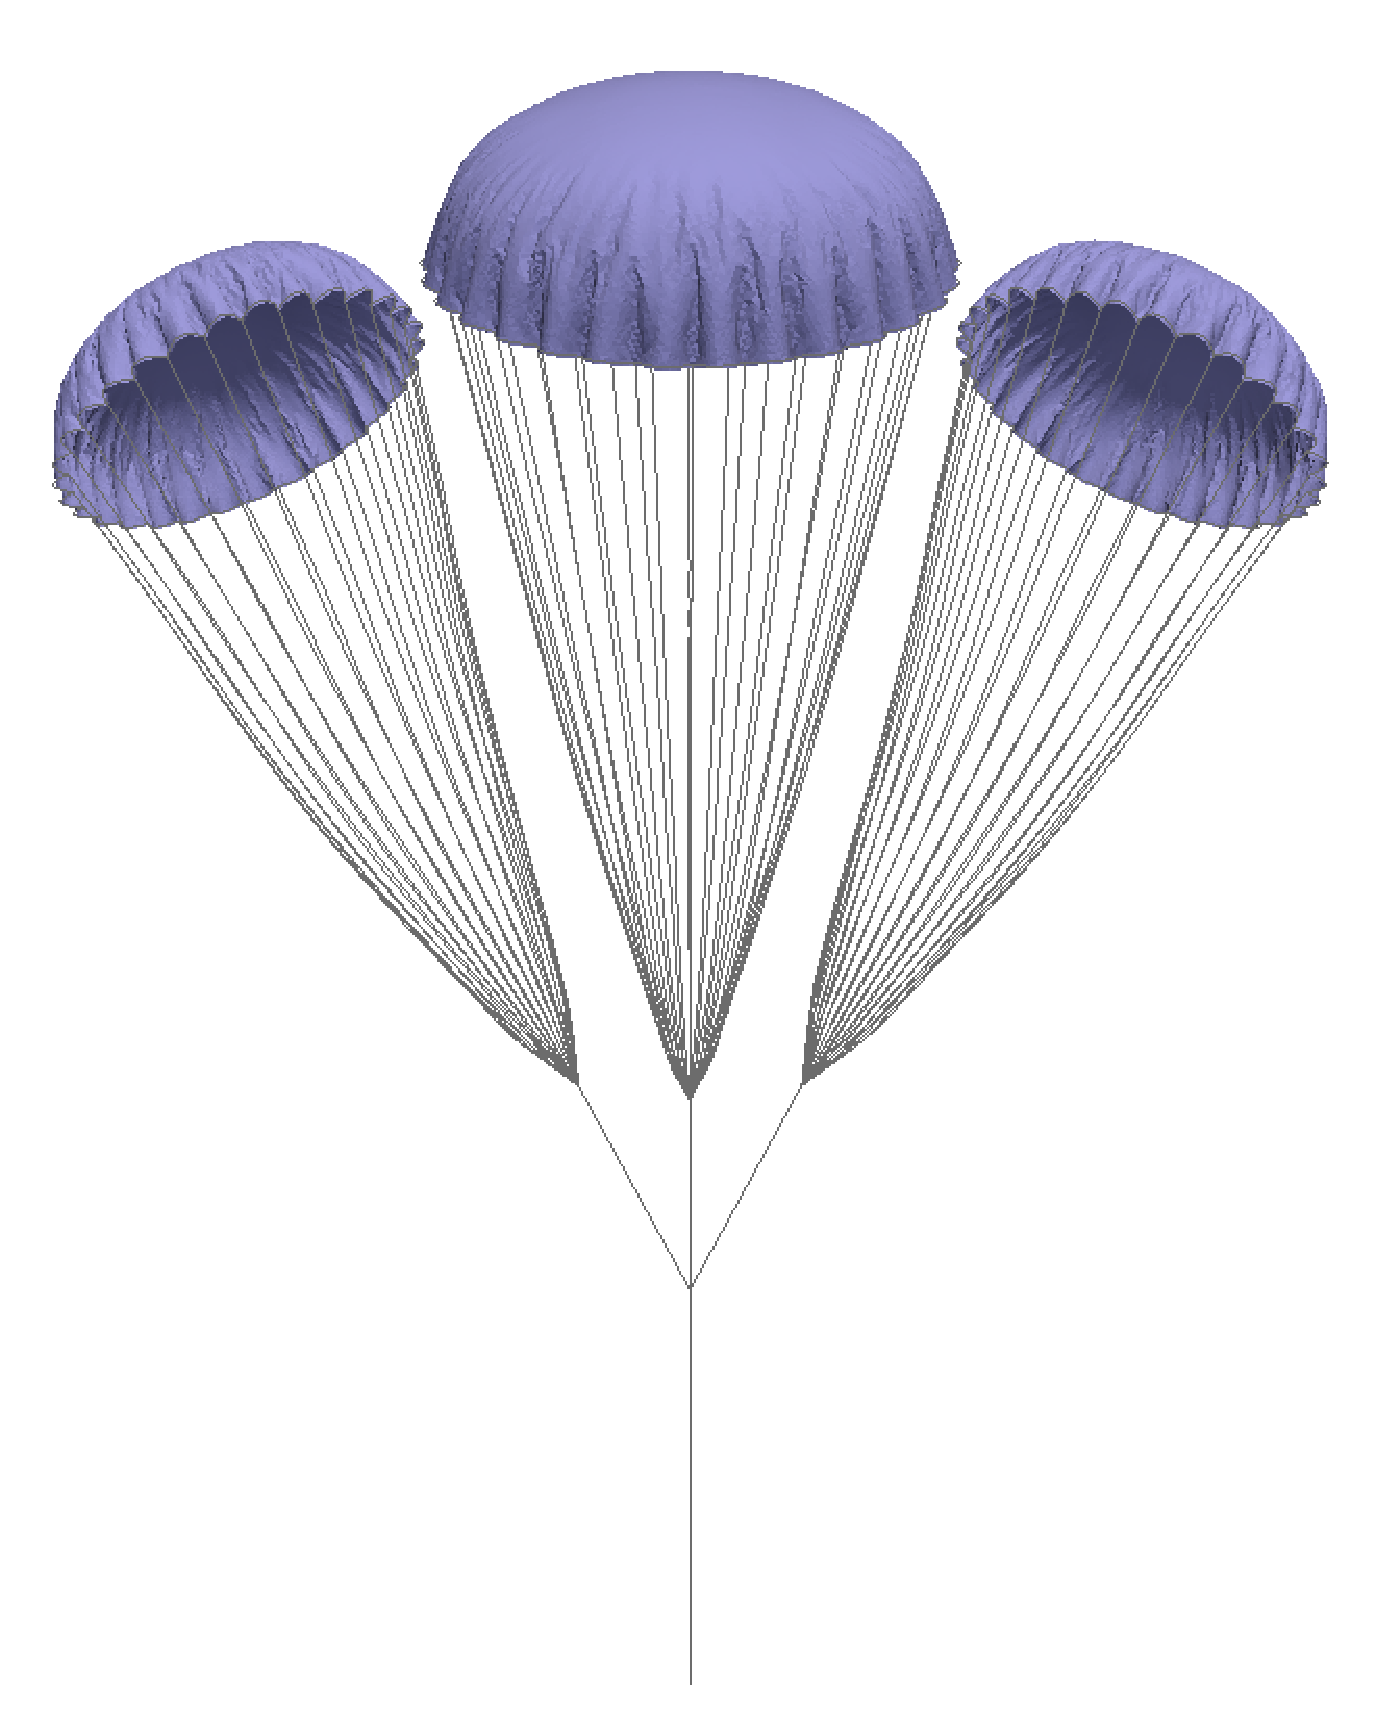
\includegraphics[width=0.32\textwidth]{figures/3G11_canopy}
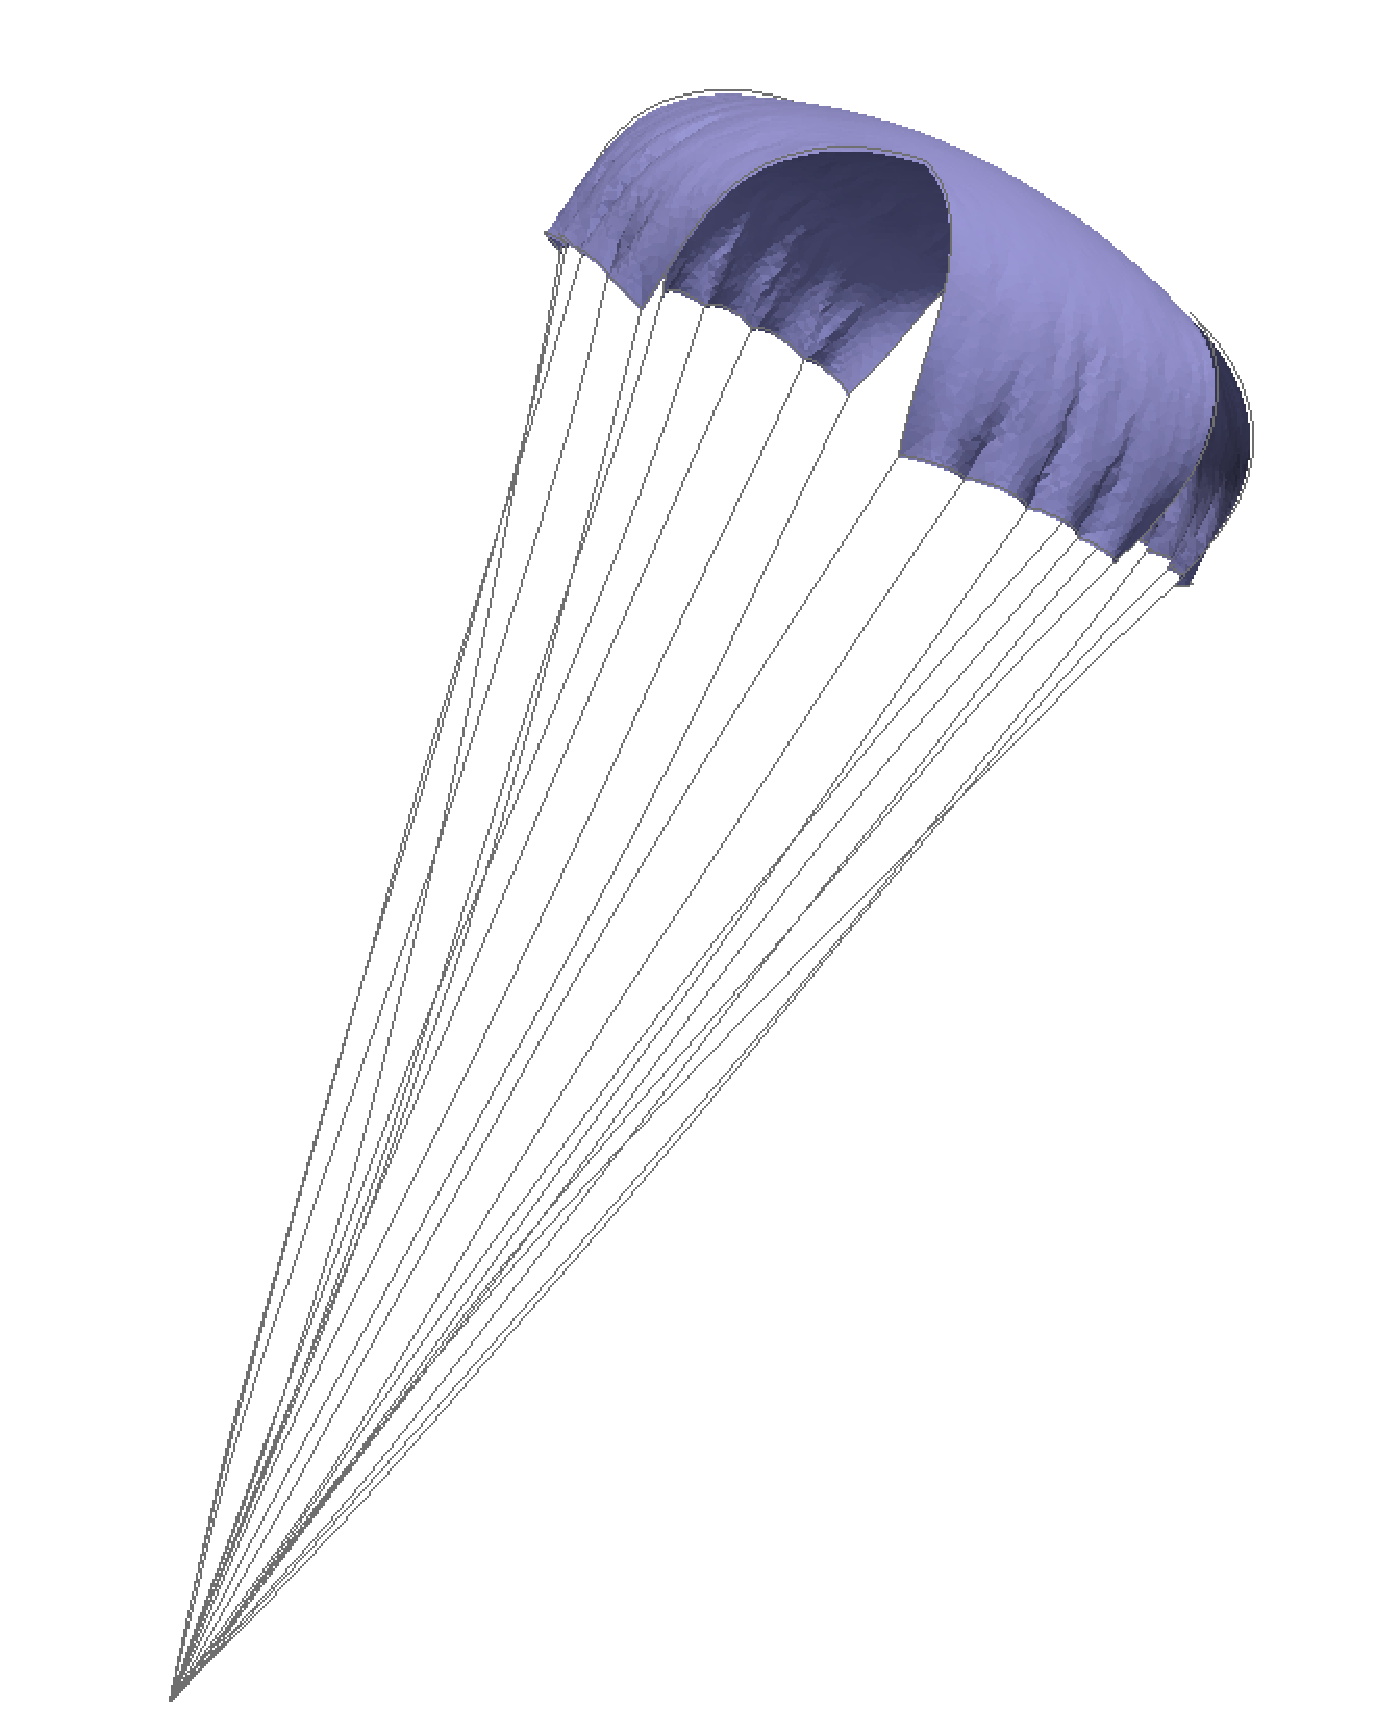
\includegraphics[width=0.32\textwidth]{figures/Cross_canopy}
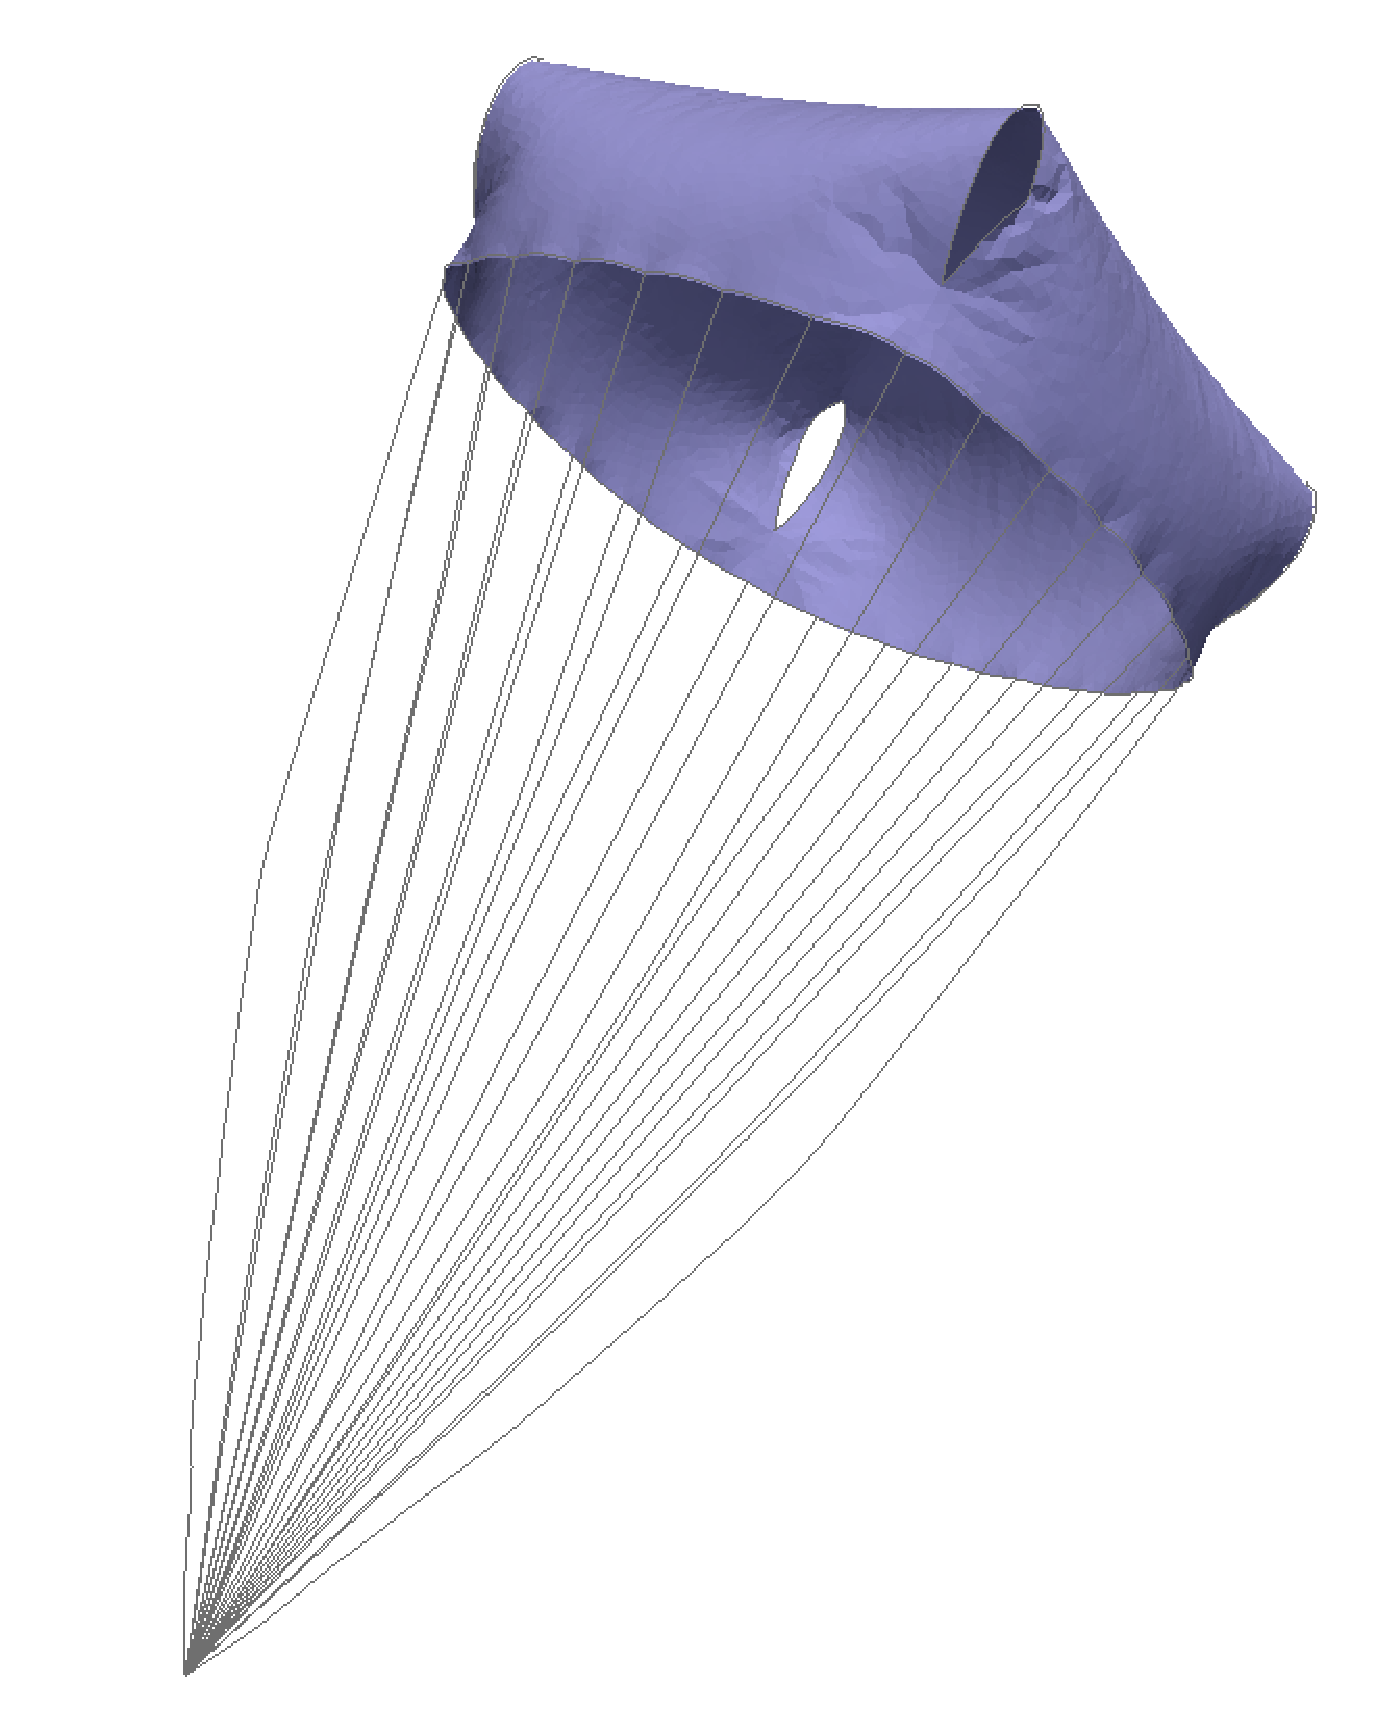
\includegraphics[width=0.32\textwidth]{figures/T11_canopy}
\caption{Three different types of parachute canopies simulated in \FronTierp
with our spring-mass model. Given parameters of a parachute, such as shape,
size, number of chords, \FronTierp has the capability to generate it.}
\label{fig:canopies}
\end{figure}

\subsection{Parachue Inflation}
Parachute inflation process is one of the most crucial stages for the
deceleration system.
In \Fig{C9_vort}, the cross-sectional velocity profile is  demonstrated at
different stages.
In this simulation, a C-9 personnel parachute with its nominal diameter
$8.53 m$ is taken as an example, and the computational domain is
$16 m\times16 m\times36 m$ with constant upward inflow velocity, outflow
boundary condition at upper outlet with pressure $p = 0$ and periodic
boundaries at the rest faces.
\begin{figure*}
\centering
\includegraphics[width=1\textwidth]{figures/C9_vort}
\caption{The cross-sectional velocity profiles around C-9 personnel
parachute during the falling process, at time $t = 1.2 s$, $t = 2.0 s$
and $t = 3.2 s$, respectively. In each plot, the left half shows the
velocity direction by arrow and the right half shows the velocity
magnitude by color, where red is large and blue is small.}
\label{fig:C9_vort}
\end{figure*}

\subsection{Wake of Parachutist}
Coupled with spring model explained in the previous sub-sections, we 
demonstrate the effect caused by the weak of the parachutist taking the 
C-9 personnel parachute (without vent) with its nominal diameter $8.53 m$ 
as an example, and set the computational domain to be 
$16 m\times16 m\times36 m$ with constant upward inflow velocity, outflow 
boundary condition at upper outlet with pressure $p = 0$ and periodic 
boundaries at the rest faces.
\begin{figure}[!ht]
\centering
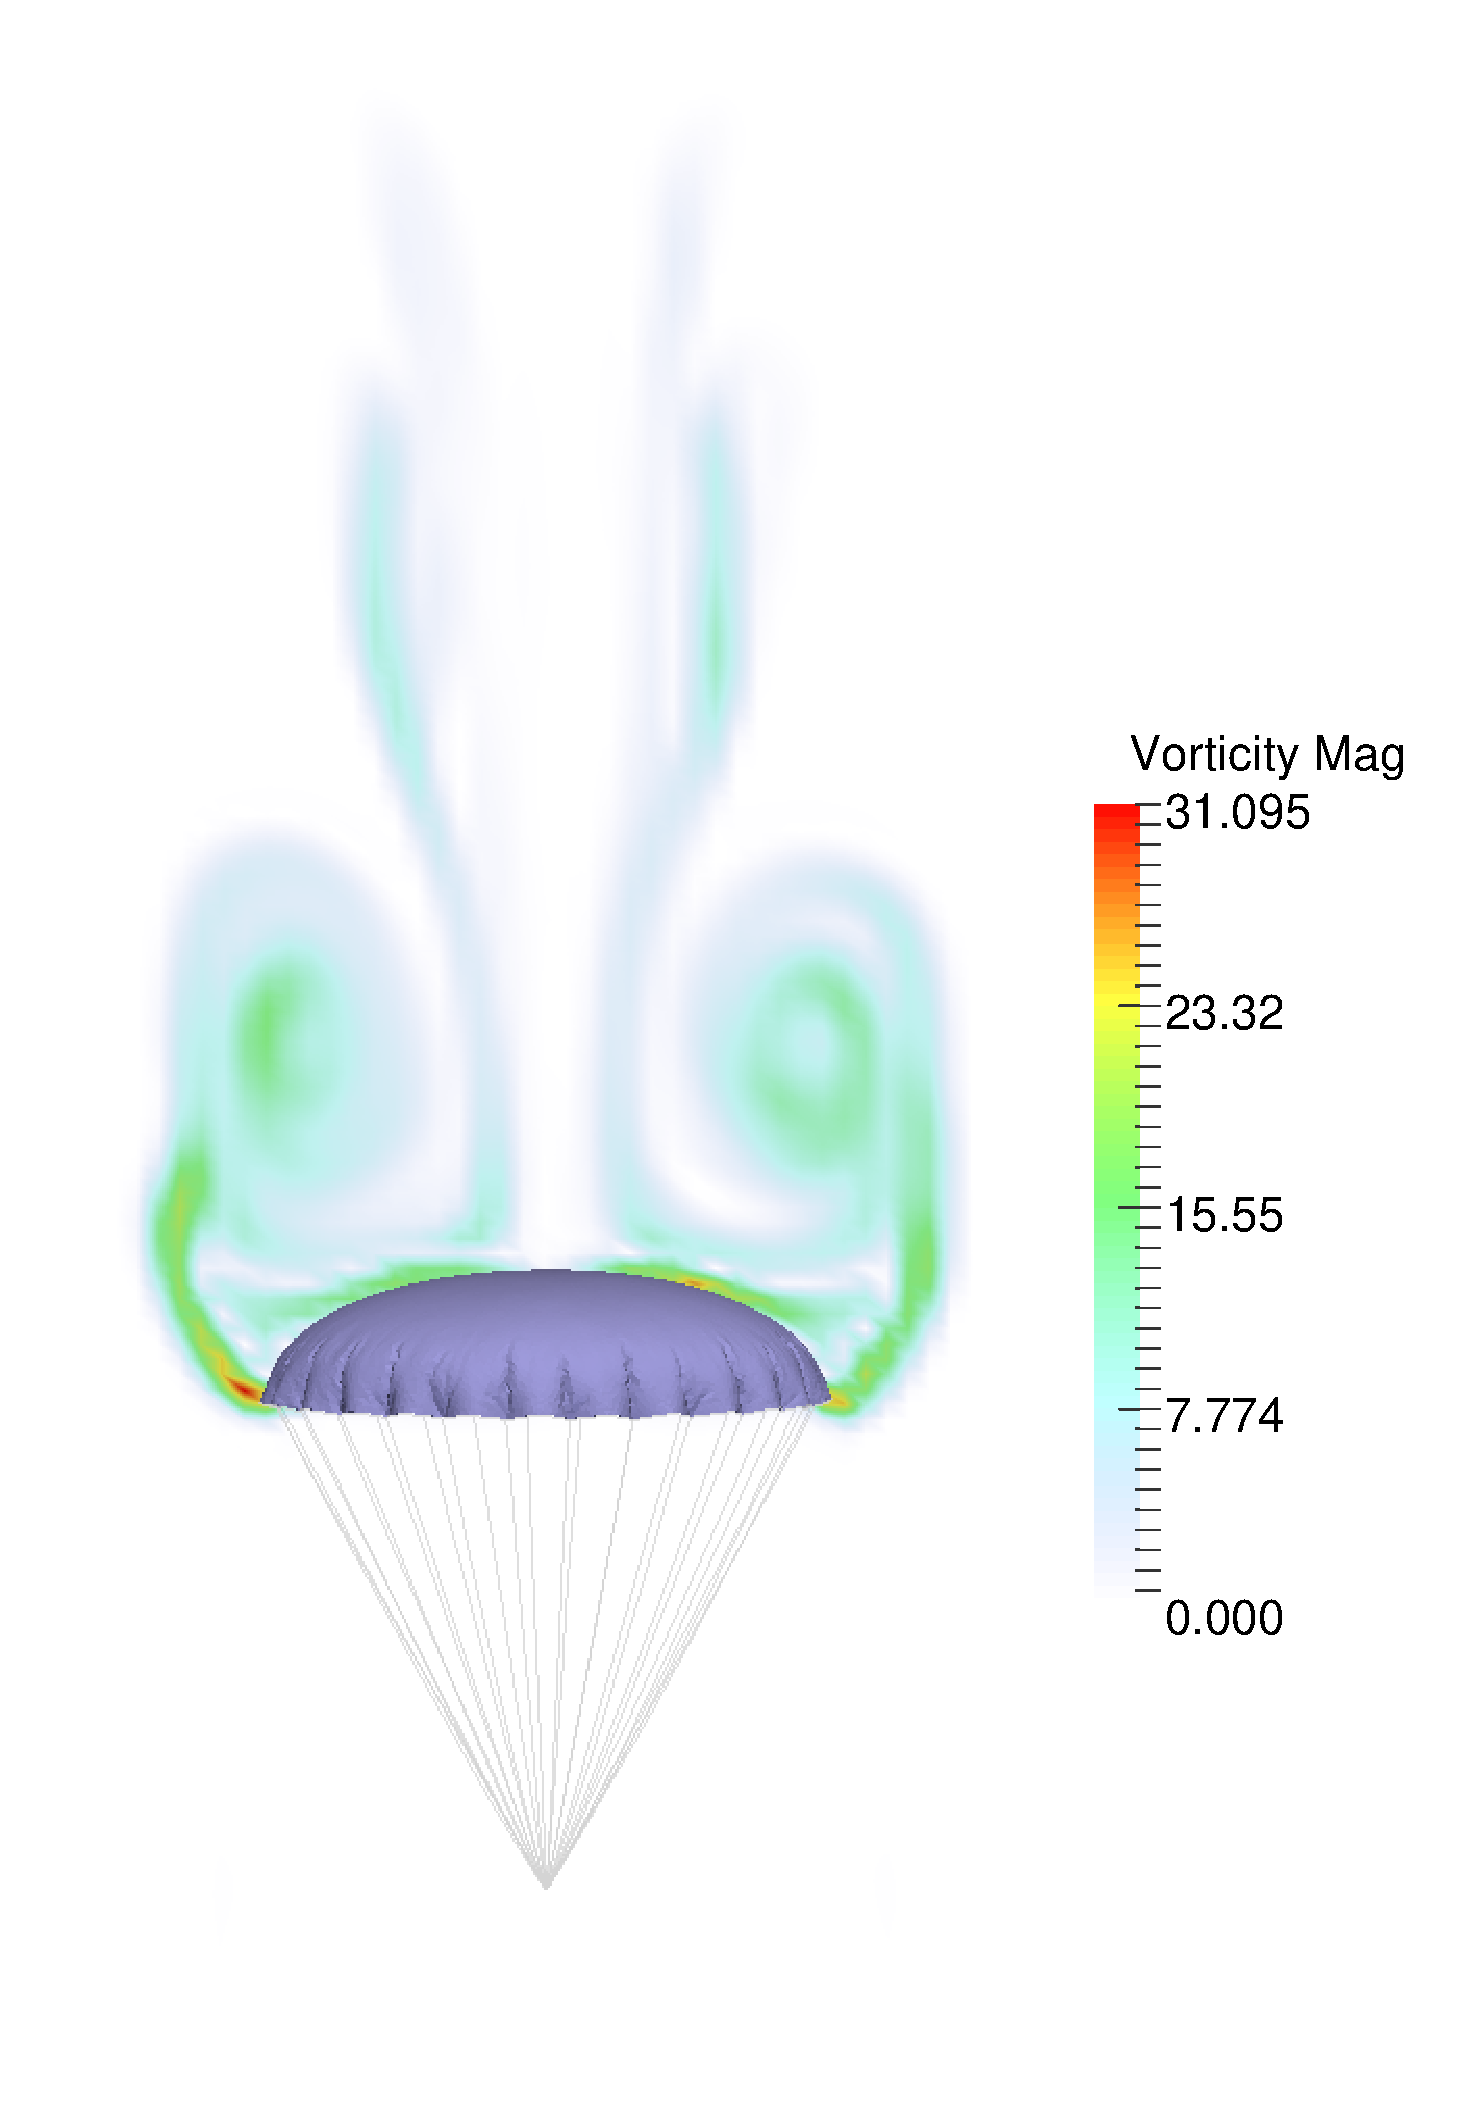
\includegraphics[width=0.48\columnwidth]{figures/C9_nohuman_vort}
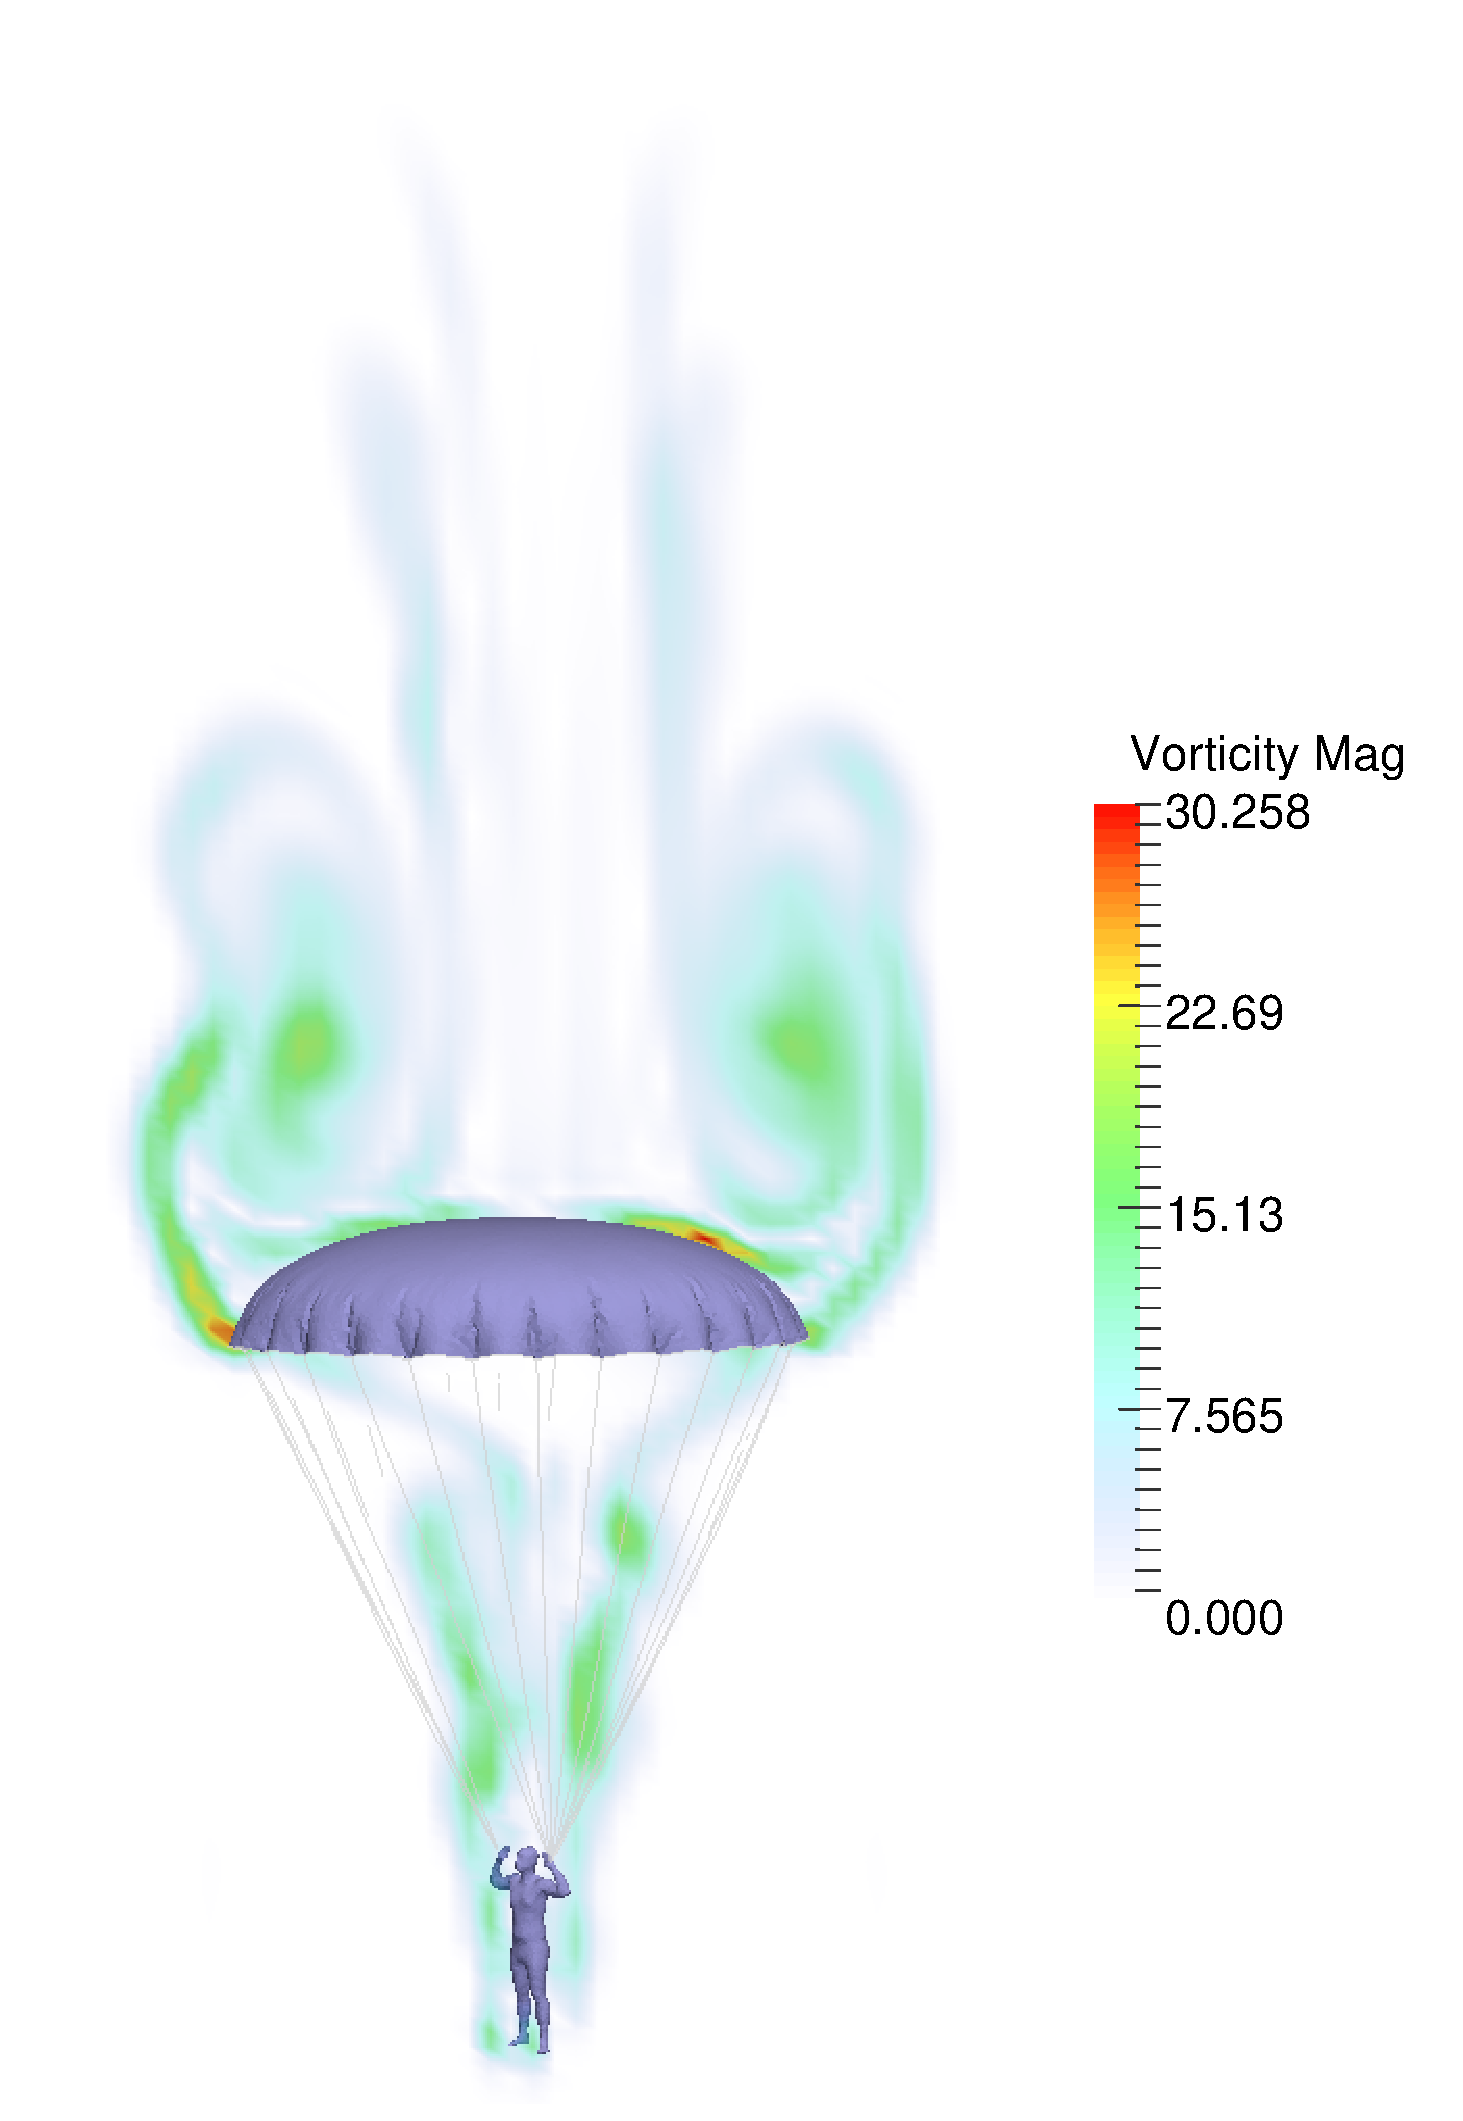
\includegraphics[width=0.48\columnwidth]{figures/C9_human_vort}
\caption{Comparison of the cross-sectional vorticity magnitude field. 
In the left figure, the parachutist is a mass point, while in the right 
figure, it is a rigid body with finite volume.}
\label{fig:C9_compare}
\end{figure}

Observed from \Fig{C9_compare}, there is turbulent flow as 
expected when the fluid flow passes the parachutist. 
Besides, the descent speed of the parachutist is slightly smaller when it is considered as a rigid body with finite volume. 
This is due to the interaction between the parachutist and the fluid flow, 
which generate an upward external force on it. 
Meanwhile, when the turbulent flow generated from fluid passing the 
parachutist reaches the canopy surface, it also has an upward force on the 
parachute system, and thus, reduces the descent speed.

\subsection{Uneven/Breaking Strings}
When designing a parachute, it is undesirable to have uneven suspension
lines or have some suspension lines broken at some time.
Here, we demonstrate these two cases in a wind tunnle test on a C-9 personnel
parachute with the computational domain size $12 m\times12 m\times24 m$.
The boundary conditions are set to be the same as above.
\begin{figure}[!ht]
\centering
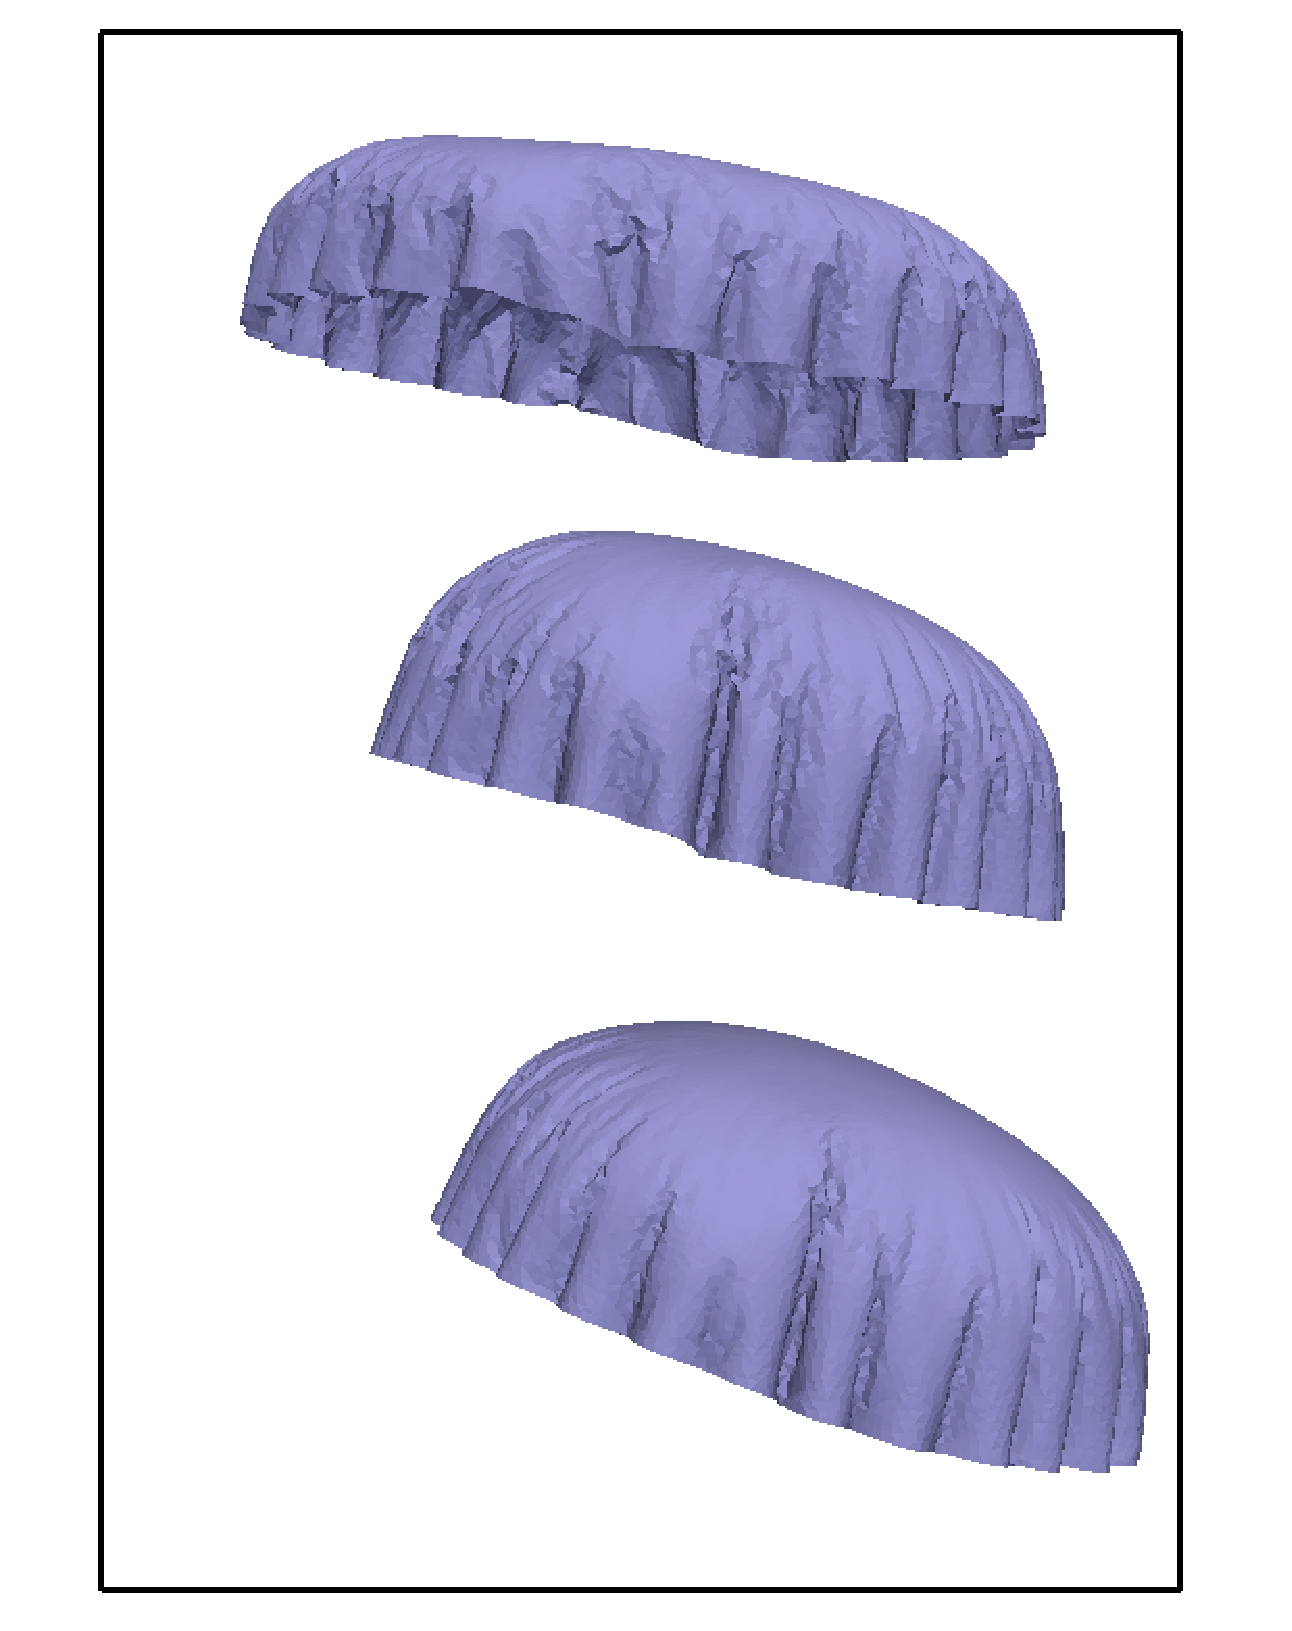
\includegraphics[width=0.48\textwidth]{figures/uneven}
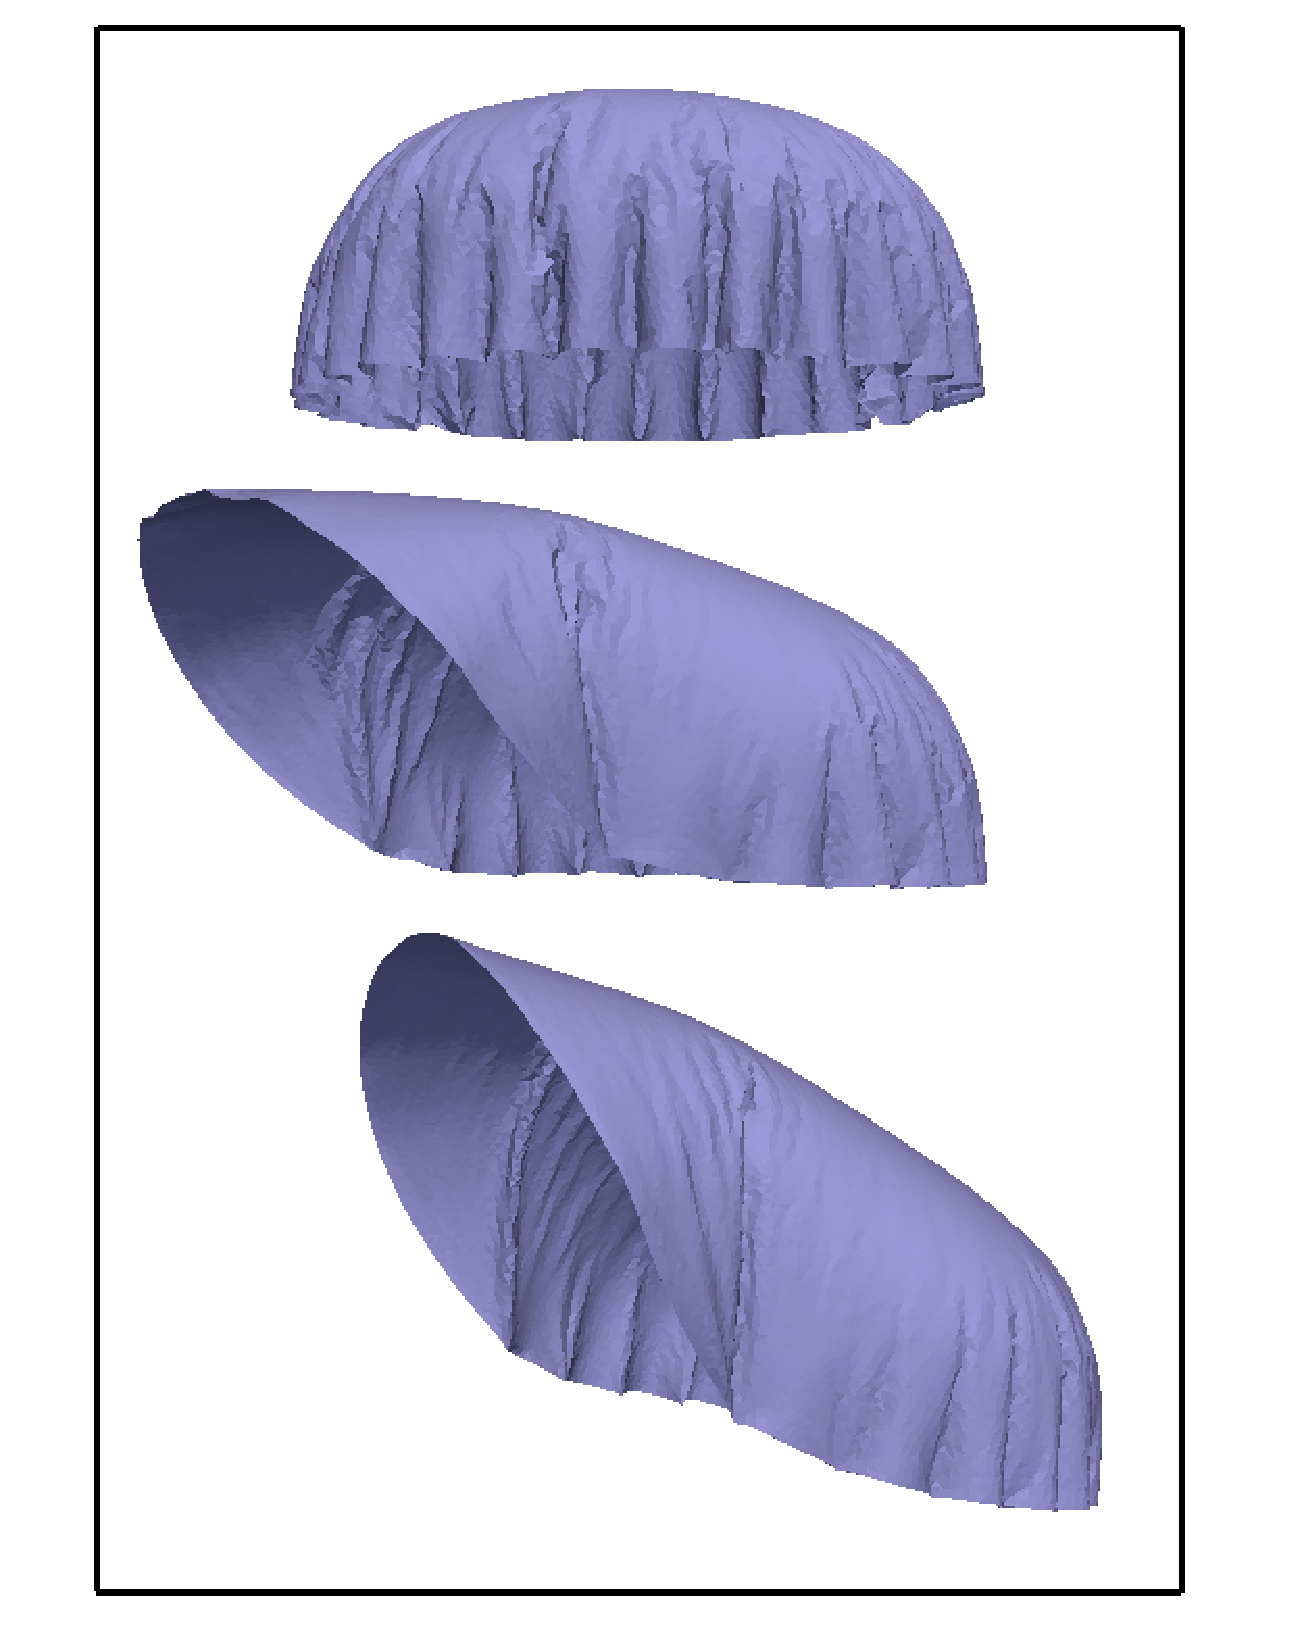
\includegraphics[width=0.48\textwidth]{figures/break}
\caption{The canopy surface of the C-9 personnel parachute at different time.
Left: 10 suspension lines are selected to have an equilibrium length than
others. Right: 10 suspension lines are selected to break at time $t = 5.0s$.}
\label{fig:uneven_break}
\end{figure}
In the left plot of \Fig{uneven_break}, 10 of the suspension lines have an
equibluim length $0.3 m$ shorter than normal which is $7 m$; while in the
right plot of \Fig{uneven_break}, 10 selected suspension lines break at
$t = 5.0s$.
Easy to observe that both cases cause the parachute canopy surface to be
unstable and lead to an angled deployment.
If the angle is too large, it could be dangerous.



\section{Collision Simulations}
As mentioned in the previous chapters, the algorithm is extended to
work for rigid bodies as well.
Since it is difficult to evaluate the correctness of cloth collision, we pay
more attention to the robustness of the algorithm.

\subsection{Benchmark: Rigid Bodies}
Because one-dimensional collisions between rigid bodies can be analytically
solved from the macro-aspect and have closed formula for velocities, we can
use this test case to demonstrate the correctness of the algorithm.
The closed formula is given by
\begin{equation}
\begin{aligned}
\widetilde{v}_a &= \frac{C_R m_b(v_b-v_a)+m_a v_a+m_b v_b}{m_a+m_b} \\
\widetilde{v}_b &= \frac{C_R m_a(v_a-v_b)+m_a v_a+m_b v_b}{m_a+m_b}
\end{aligned}
\label{eqn:rg_collsn_velo}
\end{equation}
where $C_R$ is the coefficient of restitution.
It is 1 for a complete elastic collision, and 0 for complete inelastic
collision.

Consider two cuboids initially moving toward each with velocity 0.5$m/s$ and
-0.5$m/s$ in $x$ direction, and the masses are 1$kg$ and 2$kg$, respectively.
Using formula \Eqn{rg_collsn_velo}, the speed after collision is
\begin{equation}
\begin{aligned}
\widetilde{v}_a &= -\frac{1}{6} m/s,\ 
\widetilde{v}_b = -\frac{1}{6} m/s, \mbox{ with $C_R = 0$}; \\
\widetilde{v}_a &= -\frac{5}{6} m/s,\ 
\widetilde{v}_b = \frac{1}{6} m/s,\ \mbox{ with $C_R = 1$}.
\end{aligned}
\end{equation}

\begin{figure}[!ht]
\centering
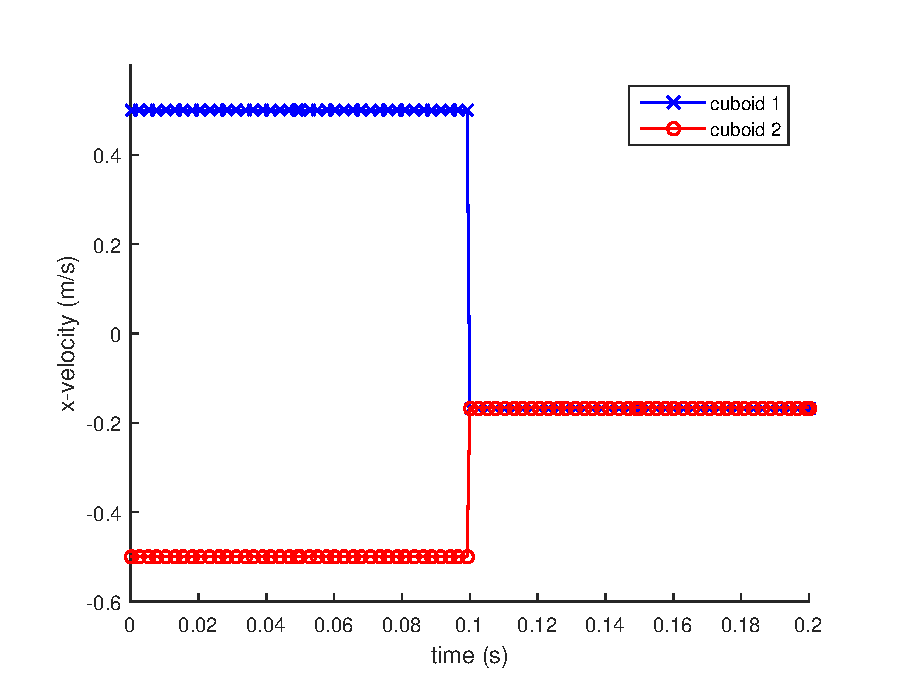
\includegraphics[width=0.48\textwidth]{figures/inelastic}
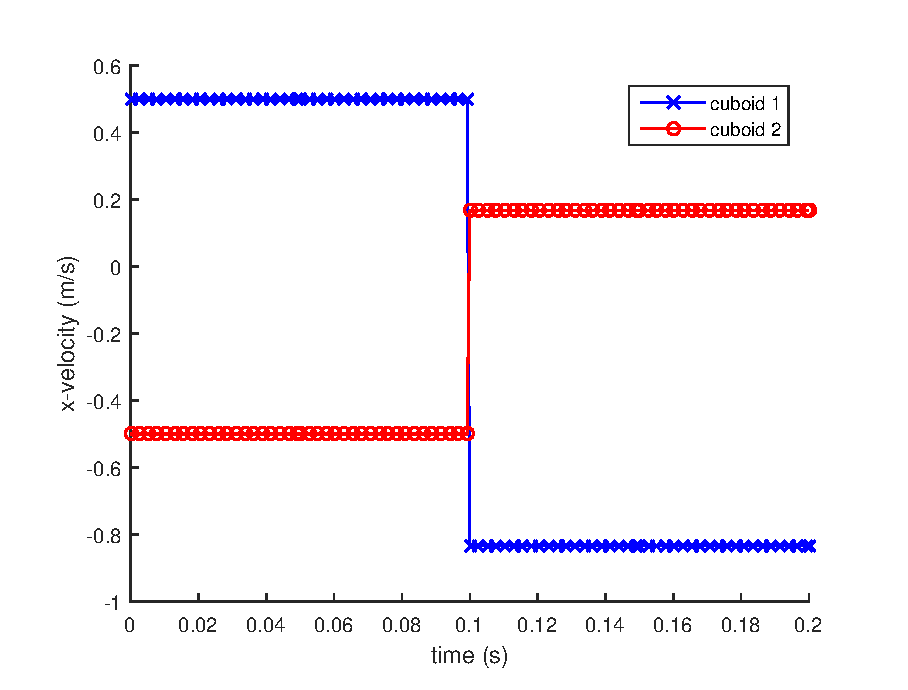
\includegraphics[width=0.48\textwidth]{figures/elastic}
\caption{The velocity profile of the two cuboids. The left figure is the
complete inelastic case ($C_R = 0$), and the right figure is the complete
elastic case ($C_R = 1$).}
\label{fig:rg_collsn_velo}
\end{figure}

\Fig{rg_collsn_velo} demonstrates the numerical profiles of
velocity in two extreme case: $C_R = 0$ and $C_R = 1$.
Clearly, it is consistent with the analytical values.
Taking complete inelastic case for example, three states of the process are
shown in \Fig{inelastic_collsn}.
\begin{figure}[!ht]
\centering
\includegraphics[width=0.32\textwidth]{figures/inelastic_0}
\includegraphics[width=0.32\textwidth]{figures/inelastic_1}
\includegraphics[width=0.32\textwidth]{figures/inelastic_2}
\caption{Complete inelastic collision. The left figure is the initial
state ($t = 0s$) and two cuboids are moving toward each other; the middle
figure is when they collide ($t = 0.1s$), after which both move to the left
with the same velocity; the right figure is the final state ($t = 1.0s$).}
\label{fig:inelastic_collsn}
\end{figure}

\subsection{Case 1: Cloth and Strings}
The first example involves the collision between elastic cloth and elastic
strings.
Initially, a flat circular cloth is right above a bunch of strings which are
straight and parallel, with their ends fixed.
Due to the gravity, cloth and strings fall and collide with each.
In this example, cloth-string collision happens first.
Then, when the cloth is folded, the strings are clustered and string-string
collision occurs.
Finally, two half parts of the cloth meet below the strings, self-collision
of cloth appears.
\Fig{fall_string} demonstrates this process, and we can observe,
all the three kinds of collision are handled properly.
\begin{figure}[!ht]
\centering
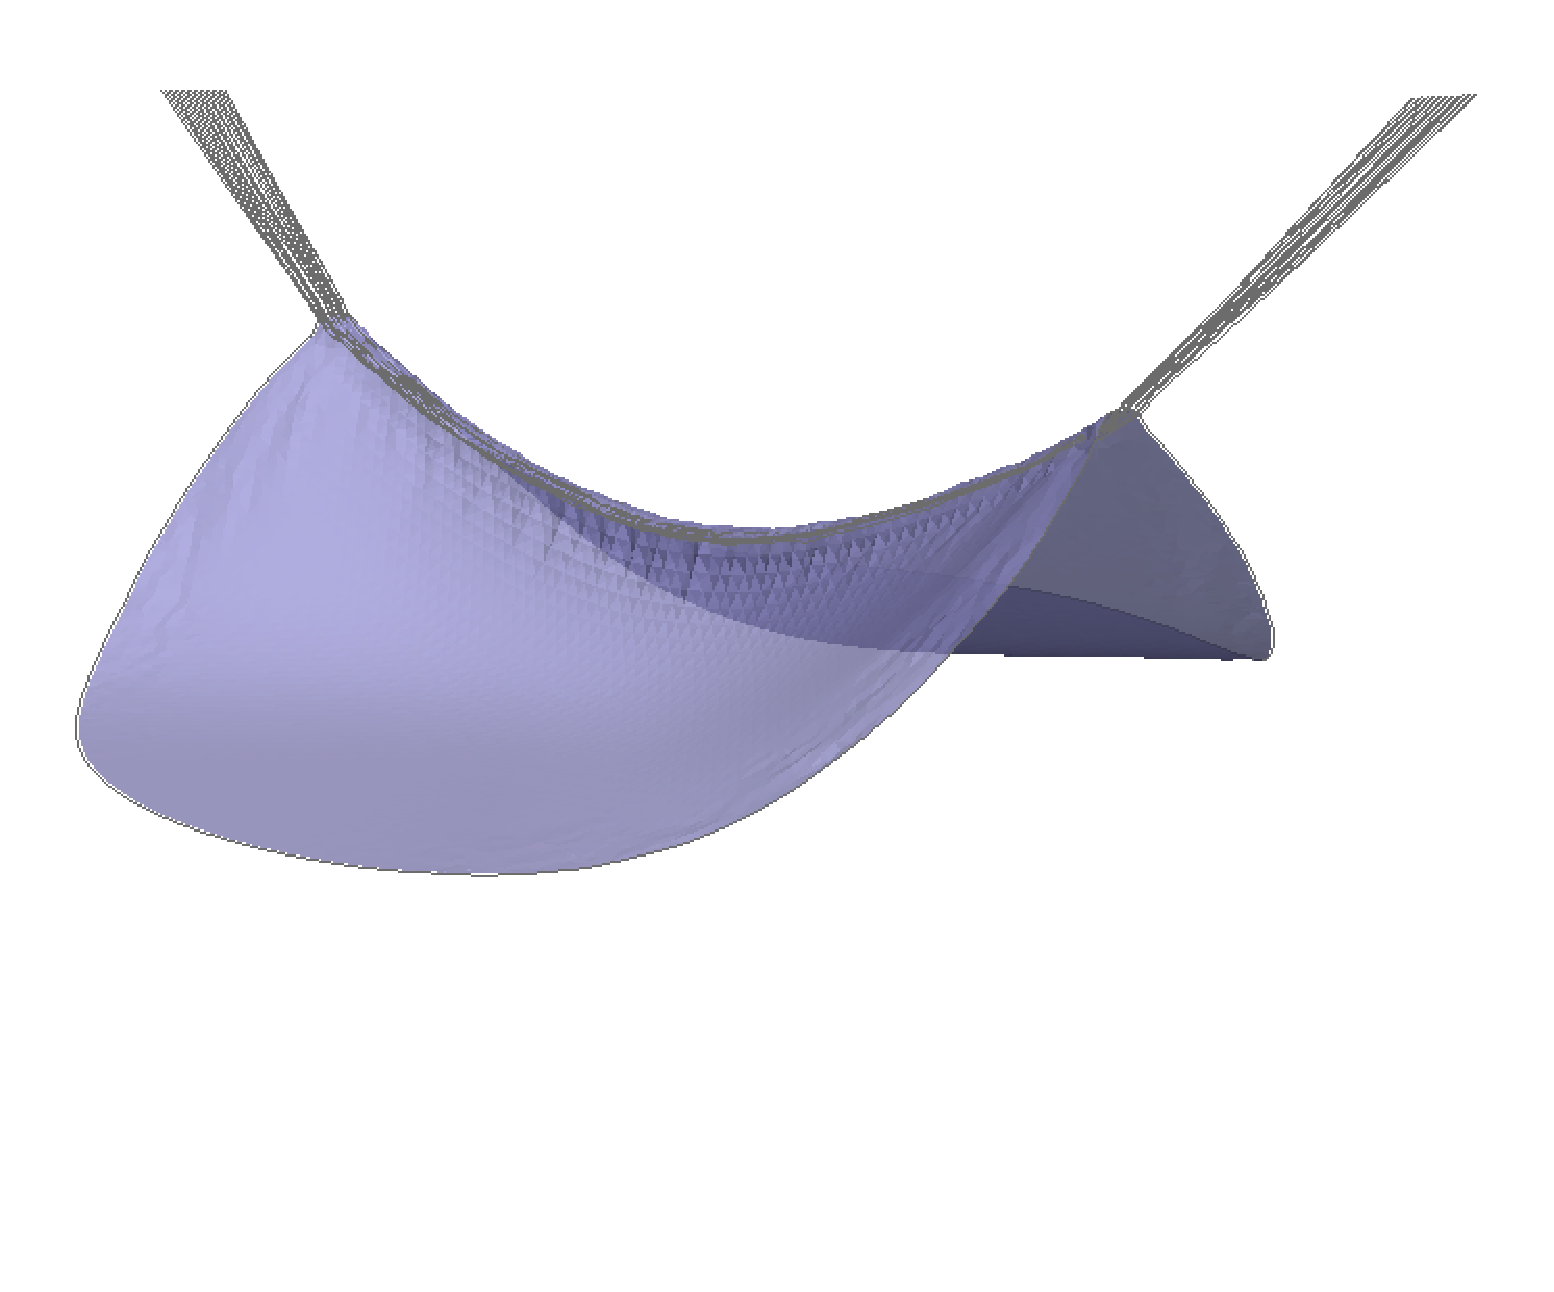
\includegraphics[width=0.48\textwidth]{figures/fall_string_0}
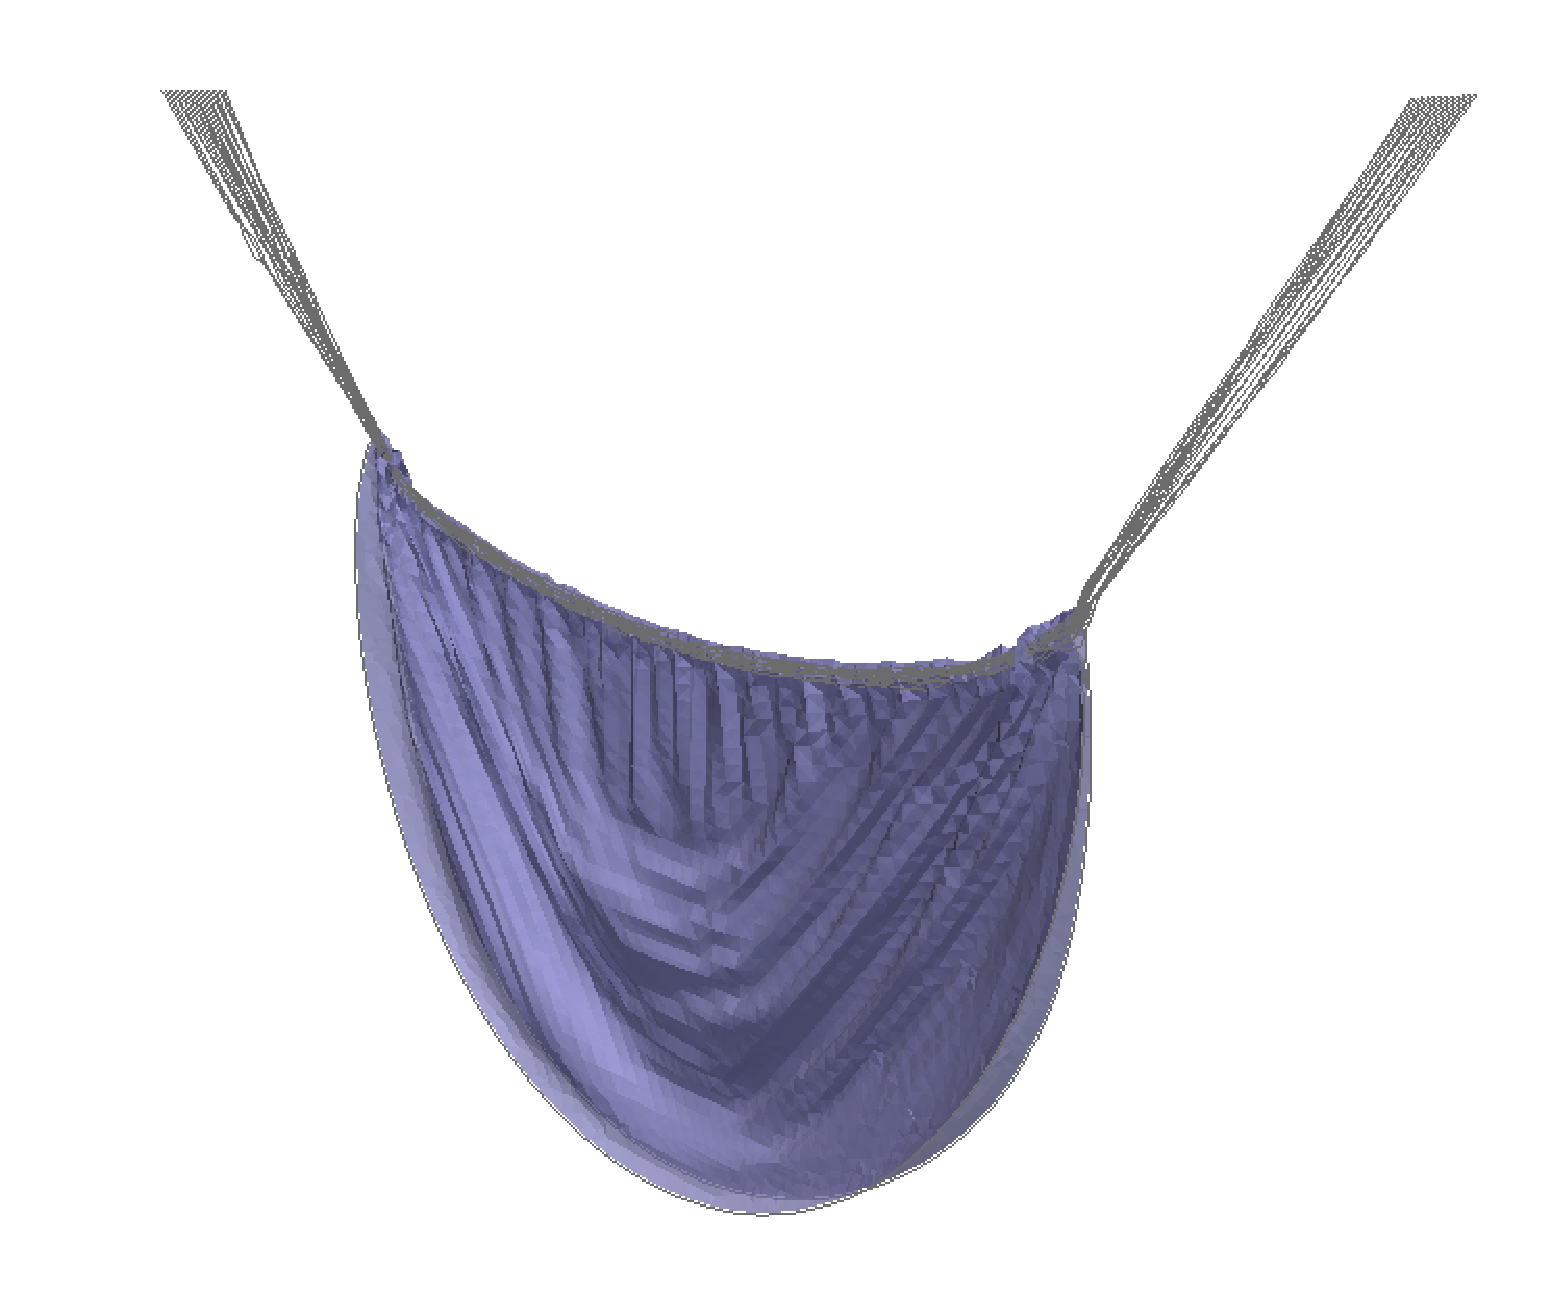
\includegraphics[width=0.48\textwidth]{figures/fall_string_1}
\caption{Two stages in the process of a circular cloth falling onto a
bunch of elastic strings. In the left figure, there are collisions between
cloth and strings. While in the right figure, the are also collisions
between the strings and self-collision of cloth.}
\label{fig:fall_string}
\end{figure}

\subsection{Case 2: Rigid Body and Cloth}
Here, we exhibit two examples demonstrating the collision between rigid
bodies and cloth.
In \Fig{rigid_cloth_collsn}, a circular fabric falls from some height
above the static cuboid object.
The bending force is taken into account in the way mentioned above. 
It highly reduces the number of collision pairs and forms the billows at
four corners.
\begin{figure}[!ht]
\centering
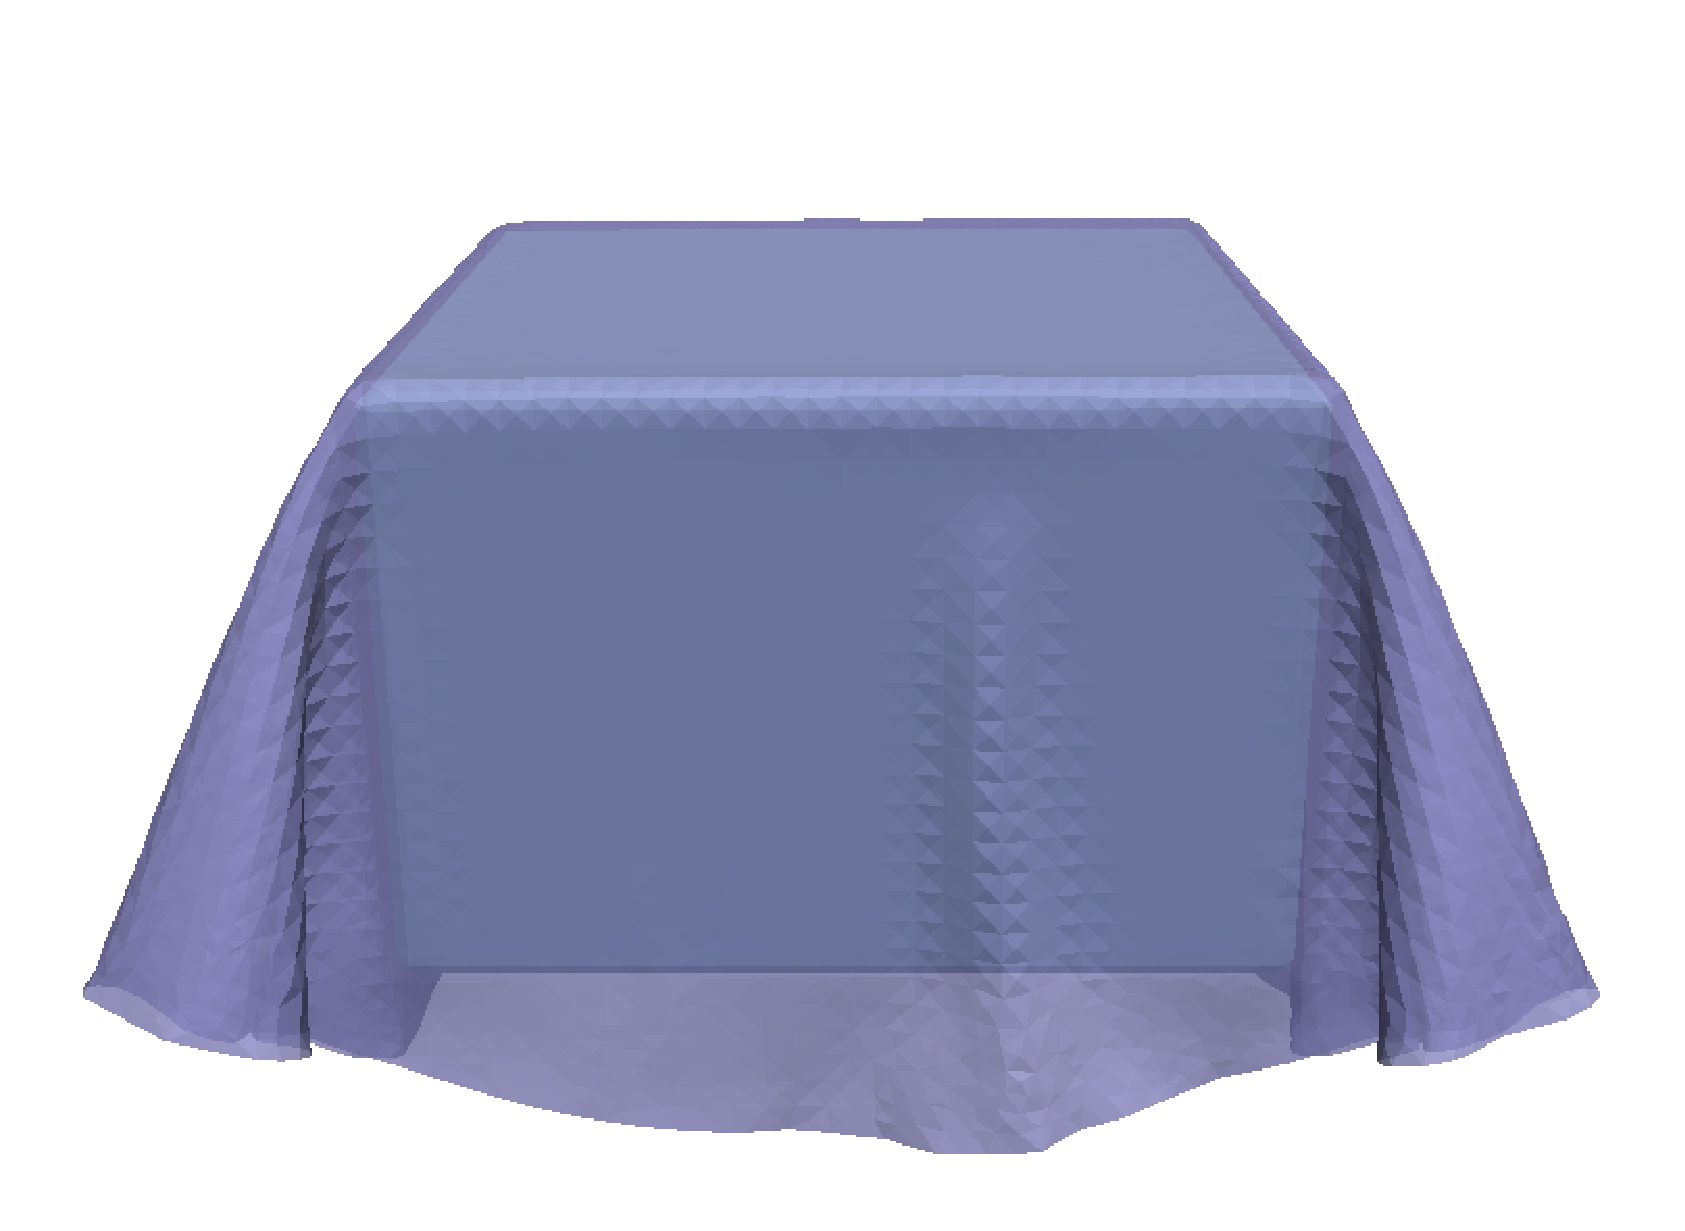
\includegraphics[width=0.48\textwidth]{figures/fall_box_0}
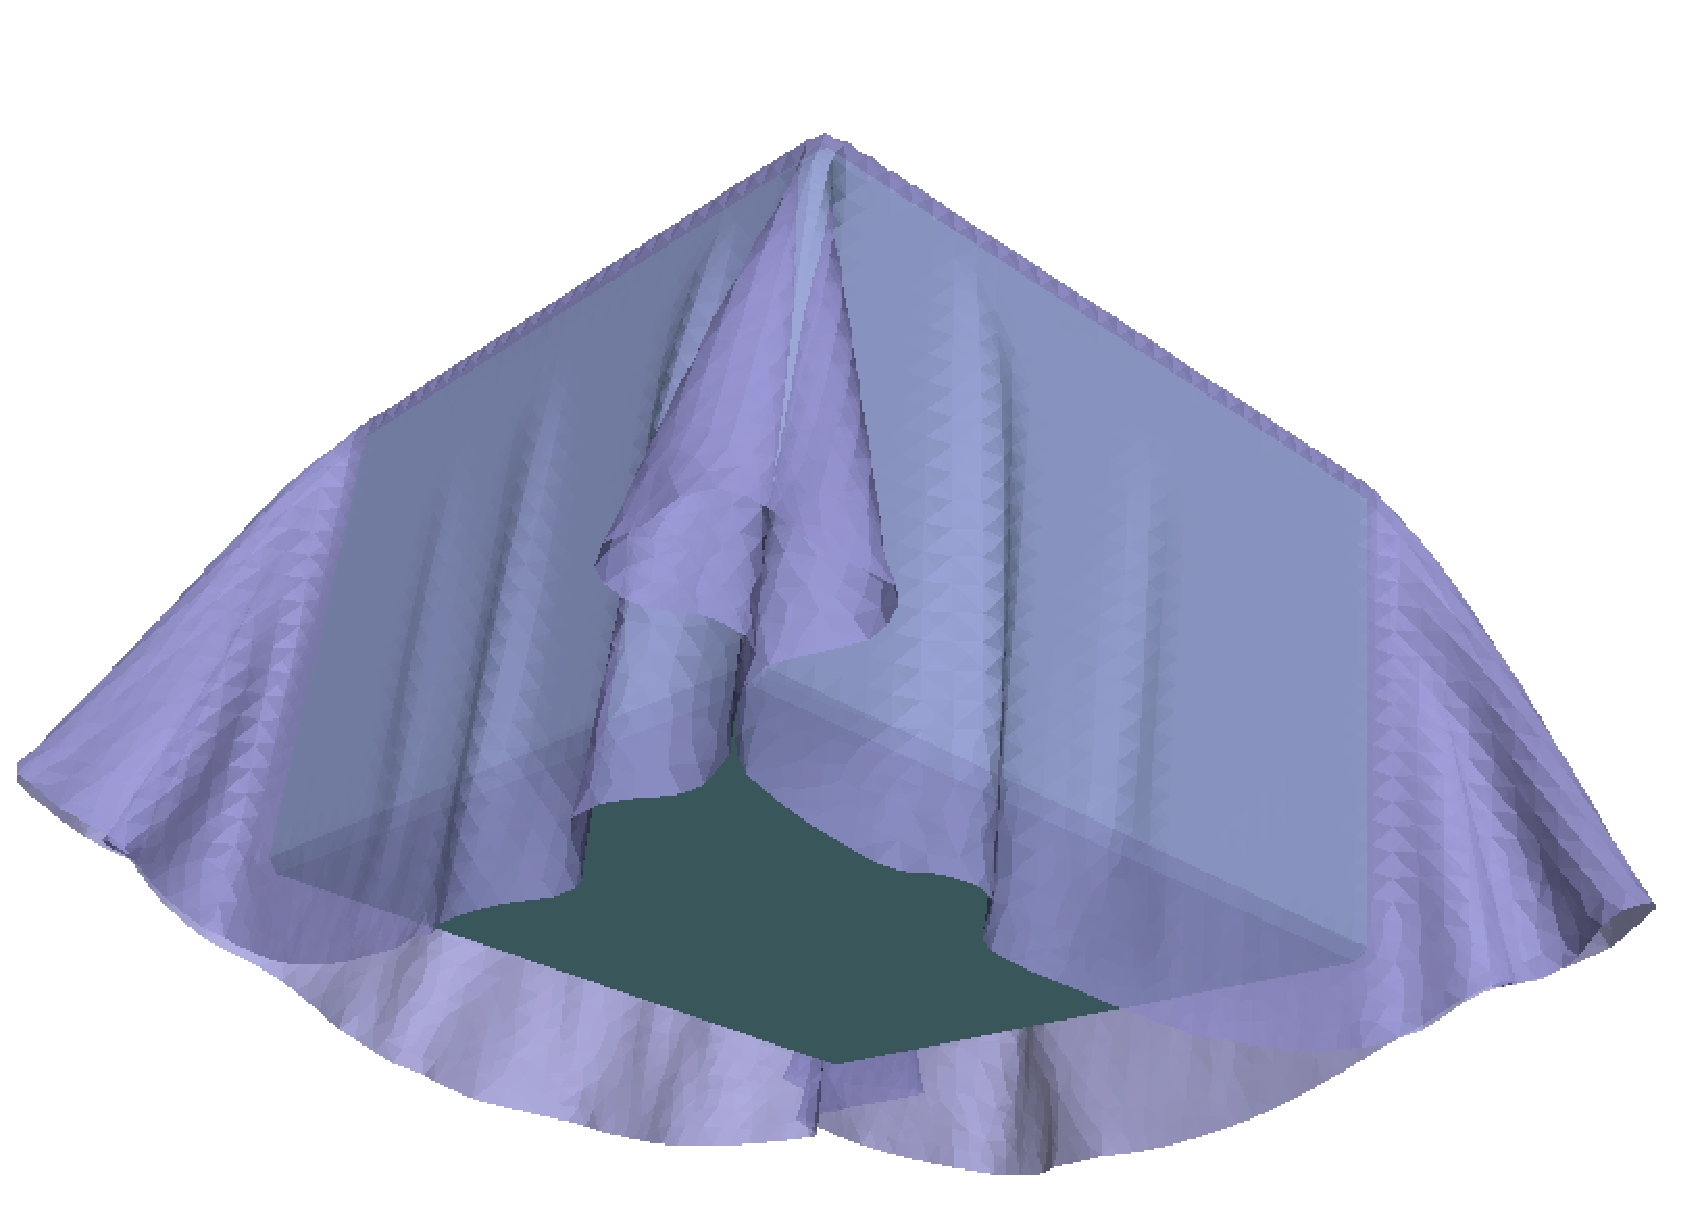
\includegraphics[width=0.48\textwidth]{figures/fall_box_1}
\caption{The front view and the side view of the cloth falling onto static
objects. Benefitted from the bending effect mentioned at the end of the
spring-mass model, billows appear at the courners.}
\label{fig:rigid_cloth_collsn}
\end{figure}

\Fig{2sphere_fall} is the falling process of two balls from some height
onto cloth with its left and right sides fixed.
In the early stage, two balls collide with the cloth, respectively, and
only rigid-elastic collision occurs.
Due to the bowl shape of the cloth, two balls are pushed towards each other
and collide at some time.
Since the collision between two balls is set to be completely inelastic,
they keep contacted and collide with the cloth together in the later stage.
\begin{figure}[!ht]
\centering
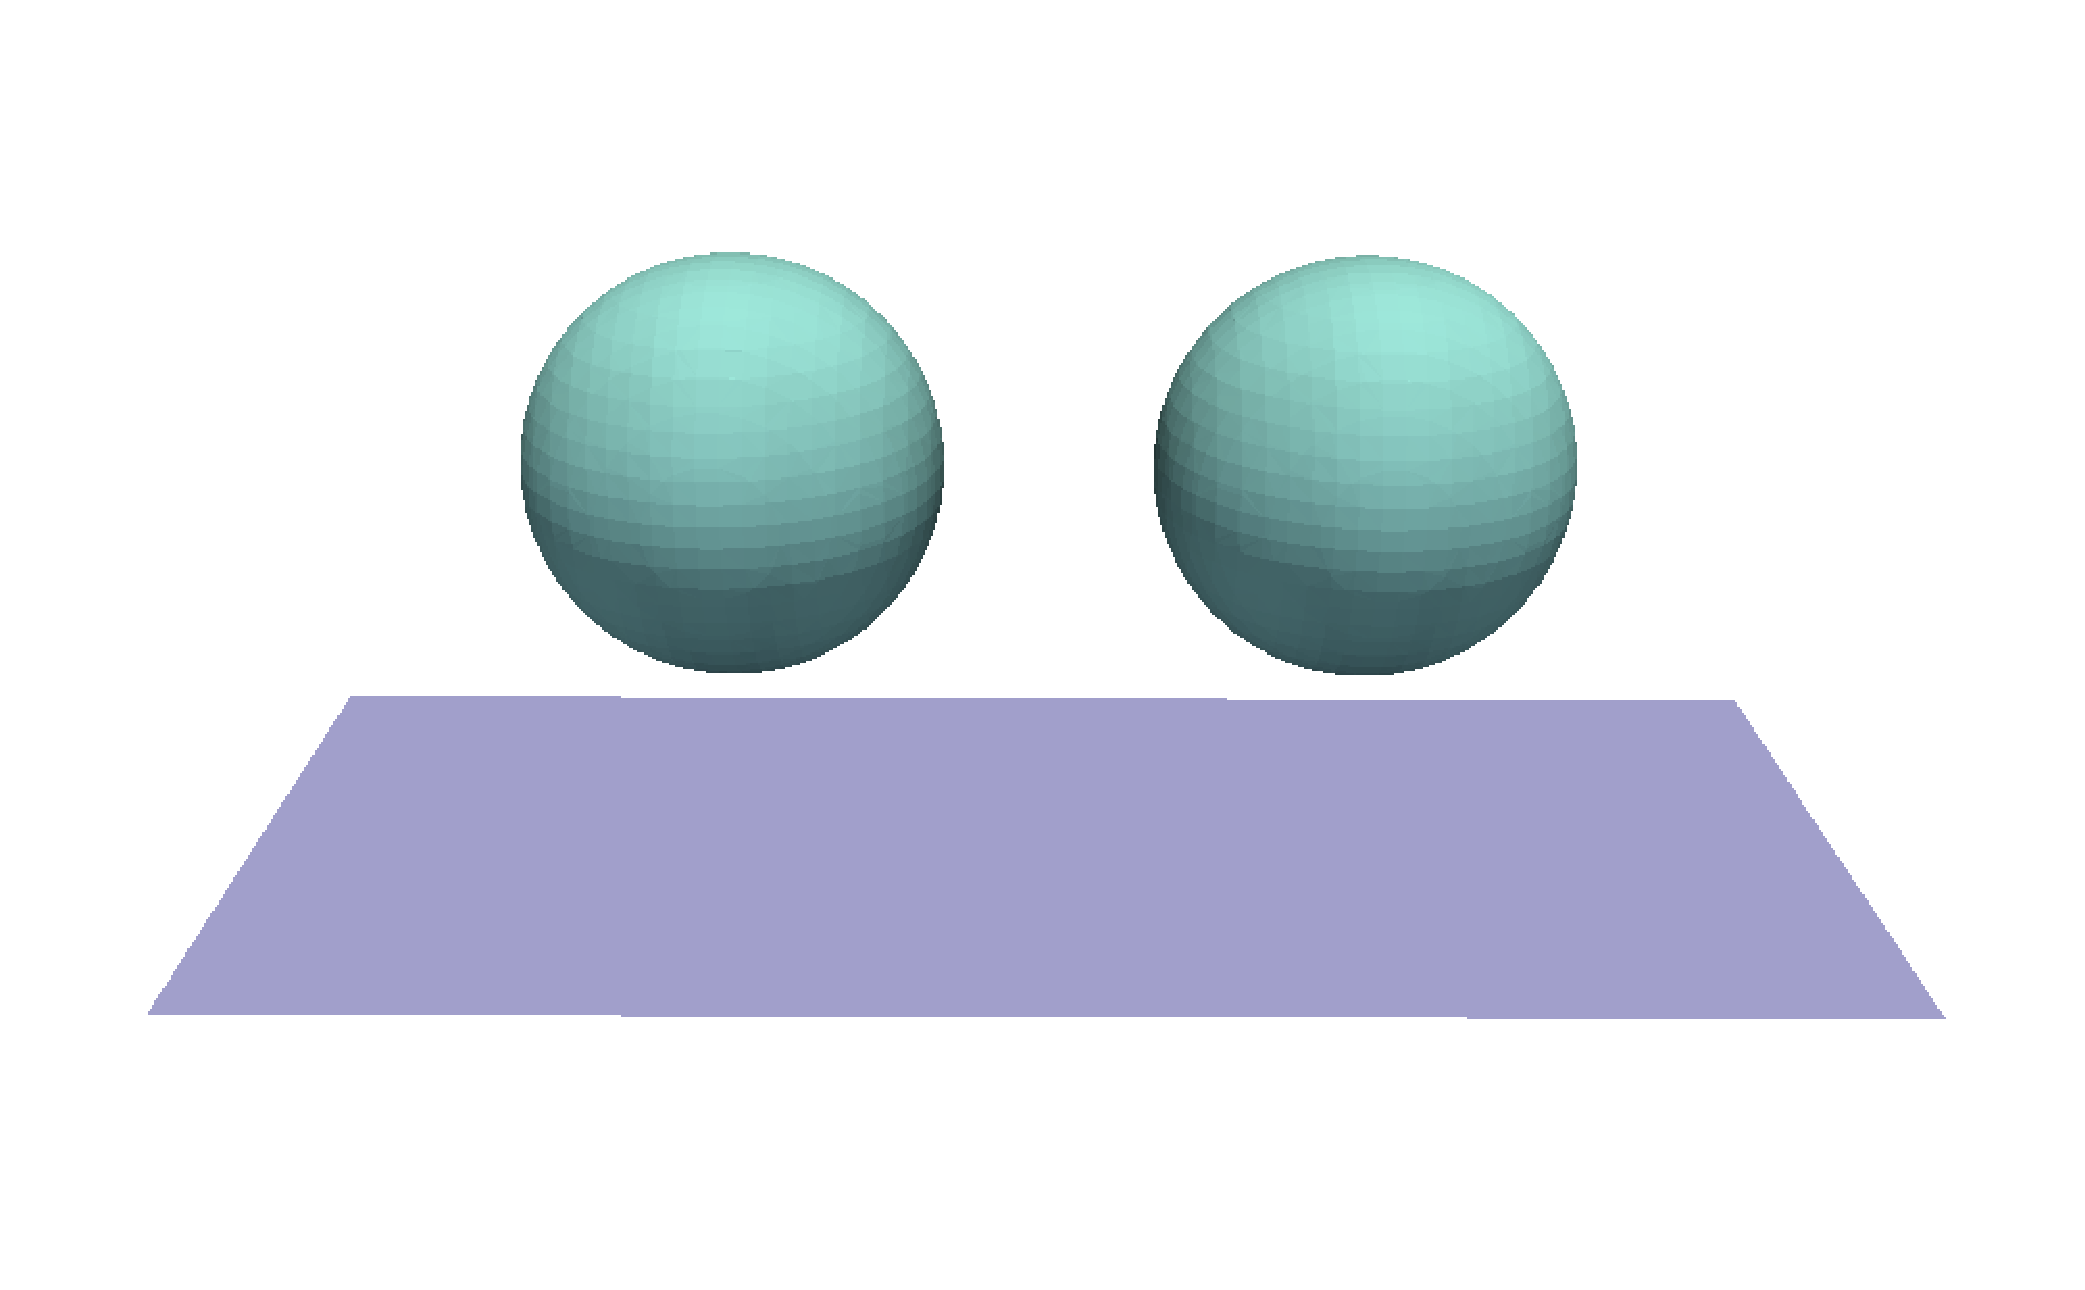
\includegraphics[width=0.48\textwidth]{figures/2sphere_fall_0}
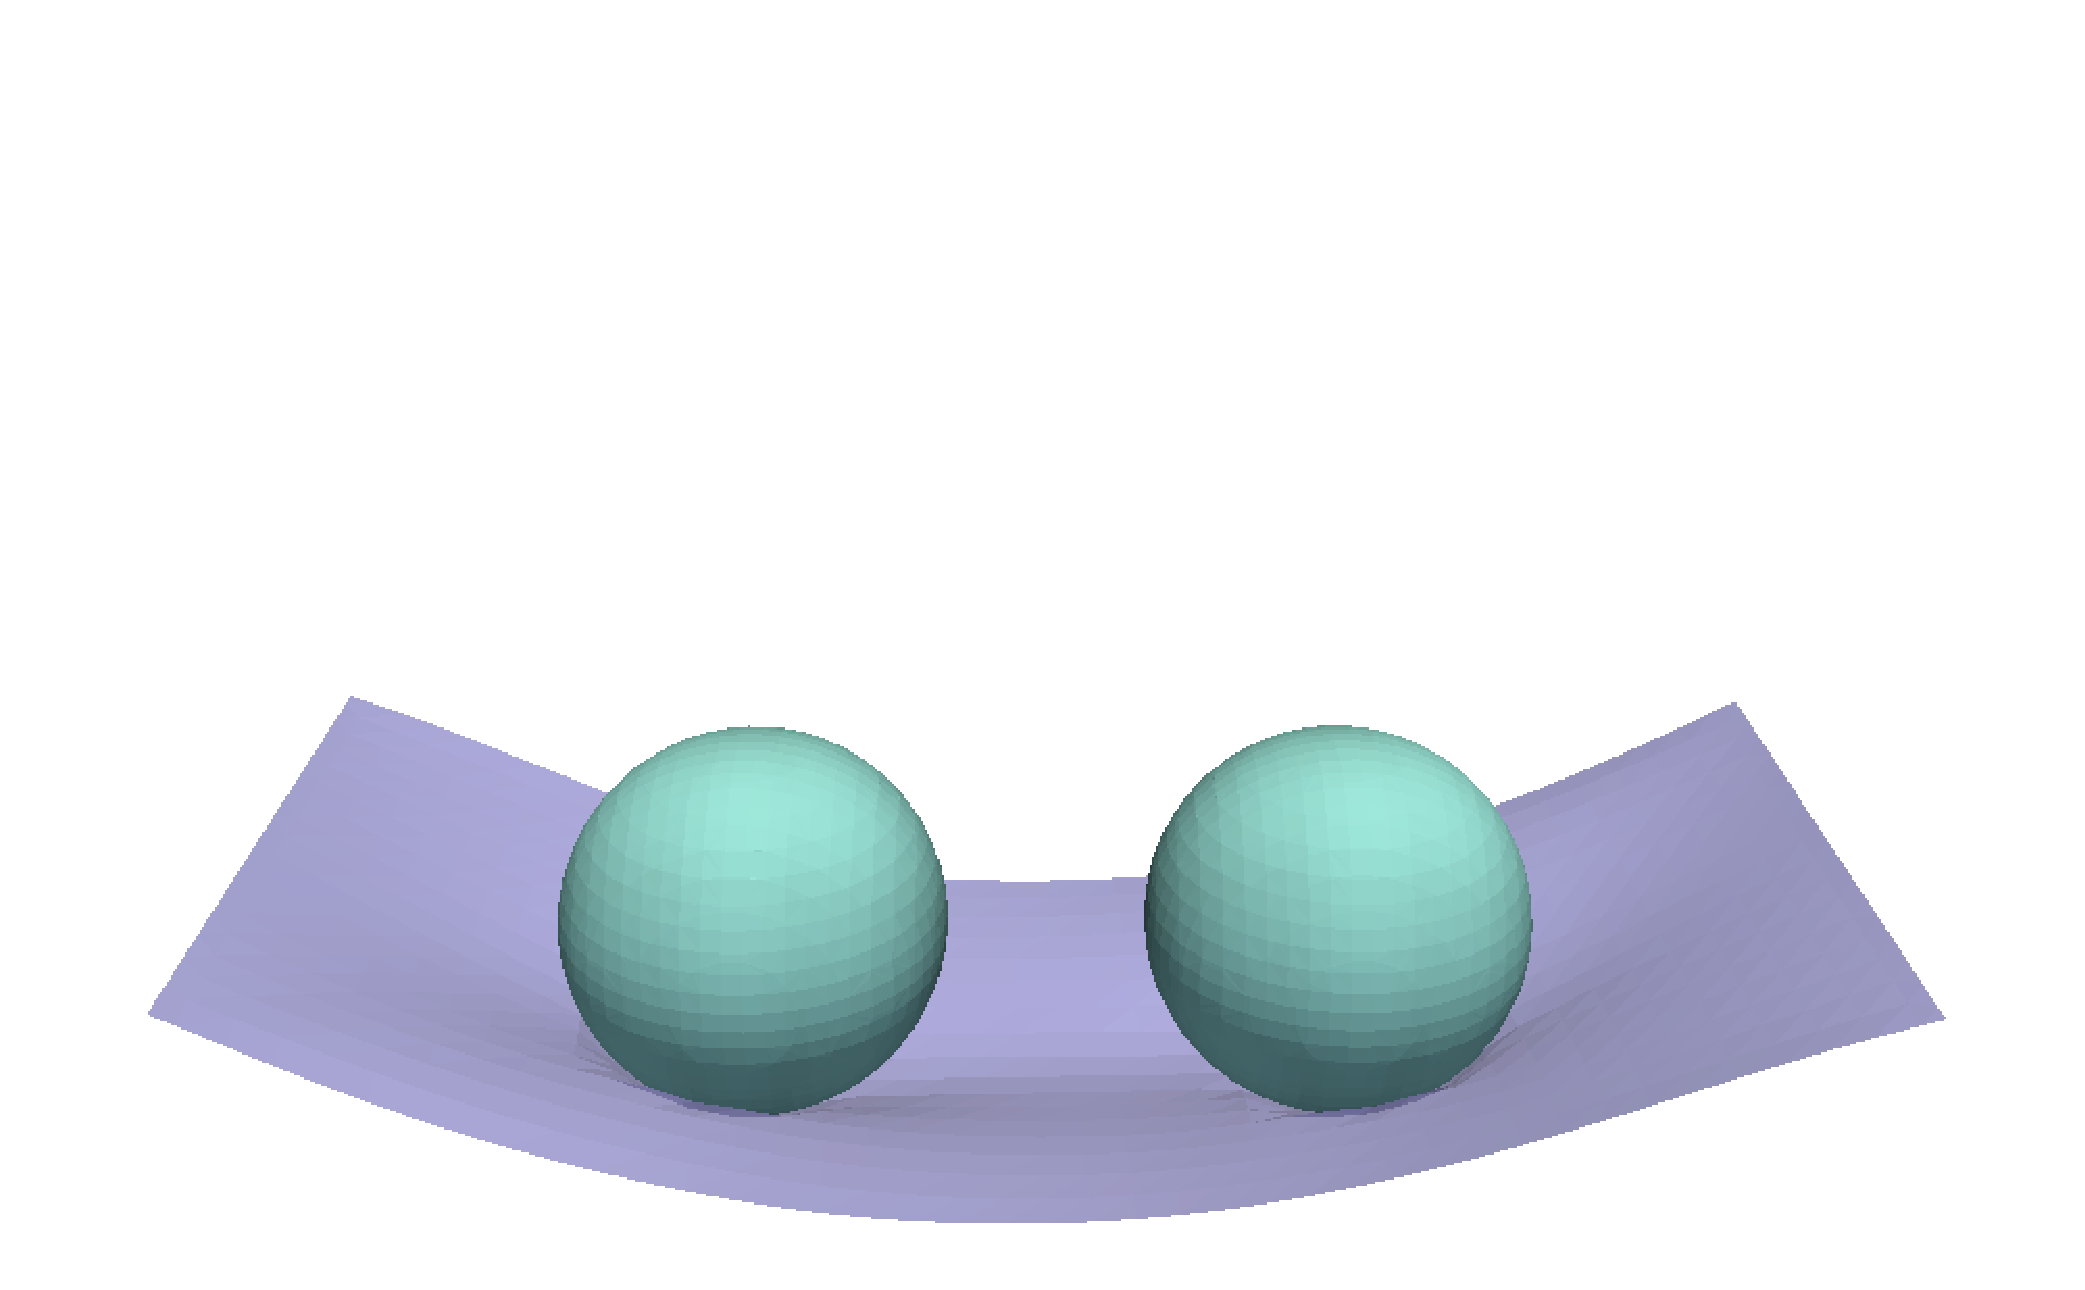
\includegraphics[width=0.48\textwidth]{figures/2sphere_fall_1} \\
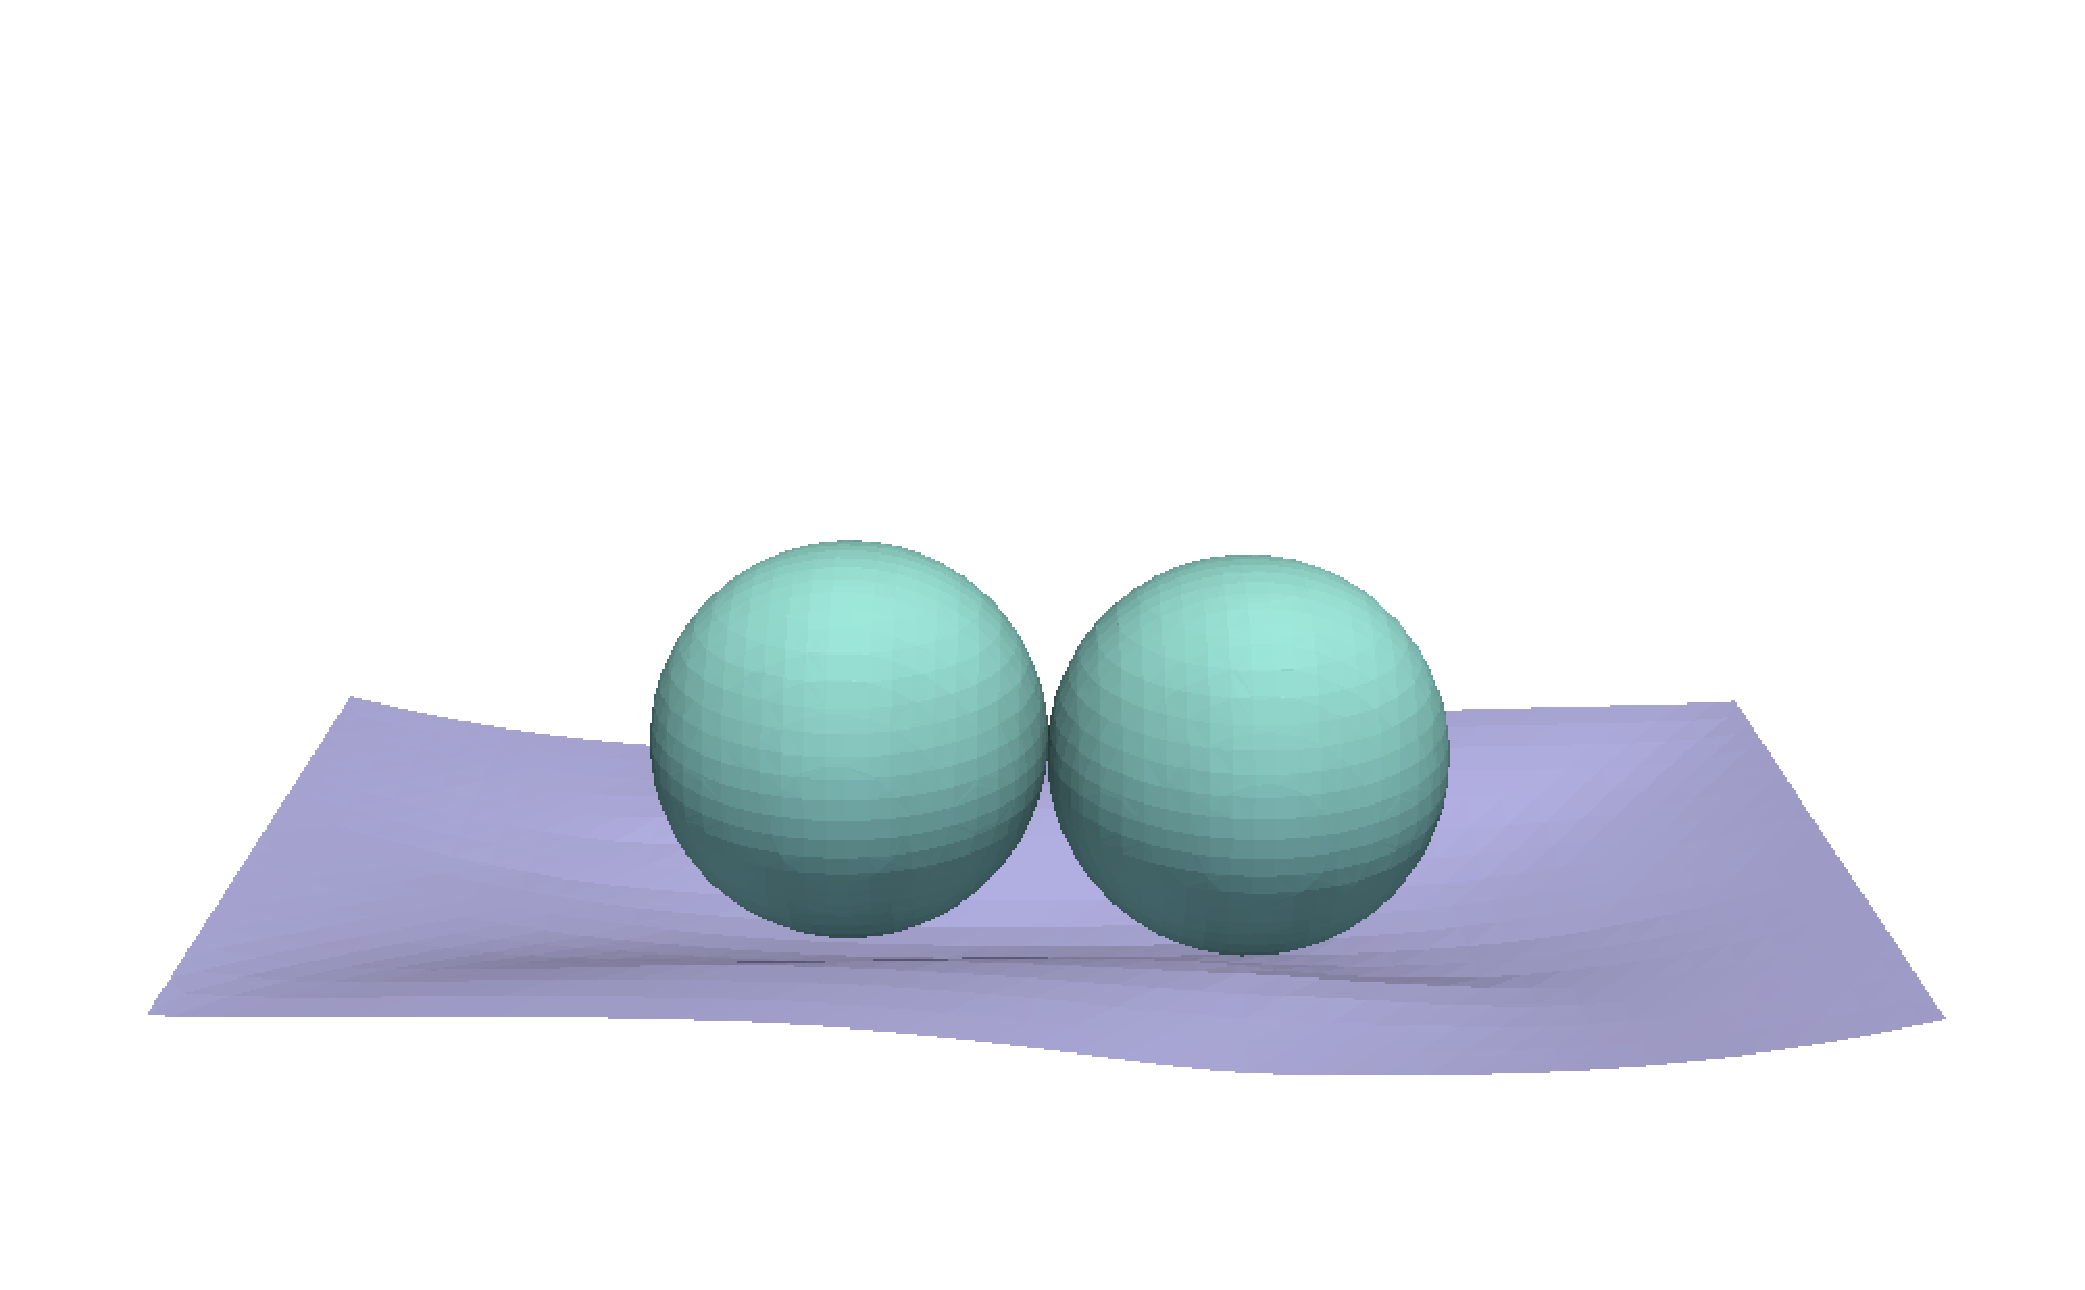
\includegraphics[width=0.48\textwidth]{figures/2sphere_fall_2}
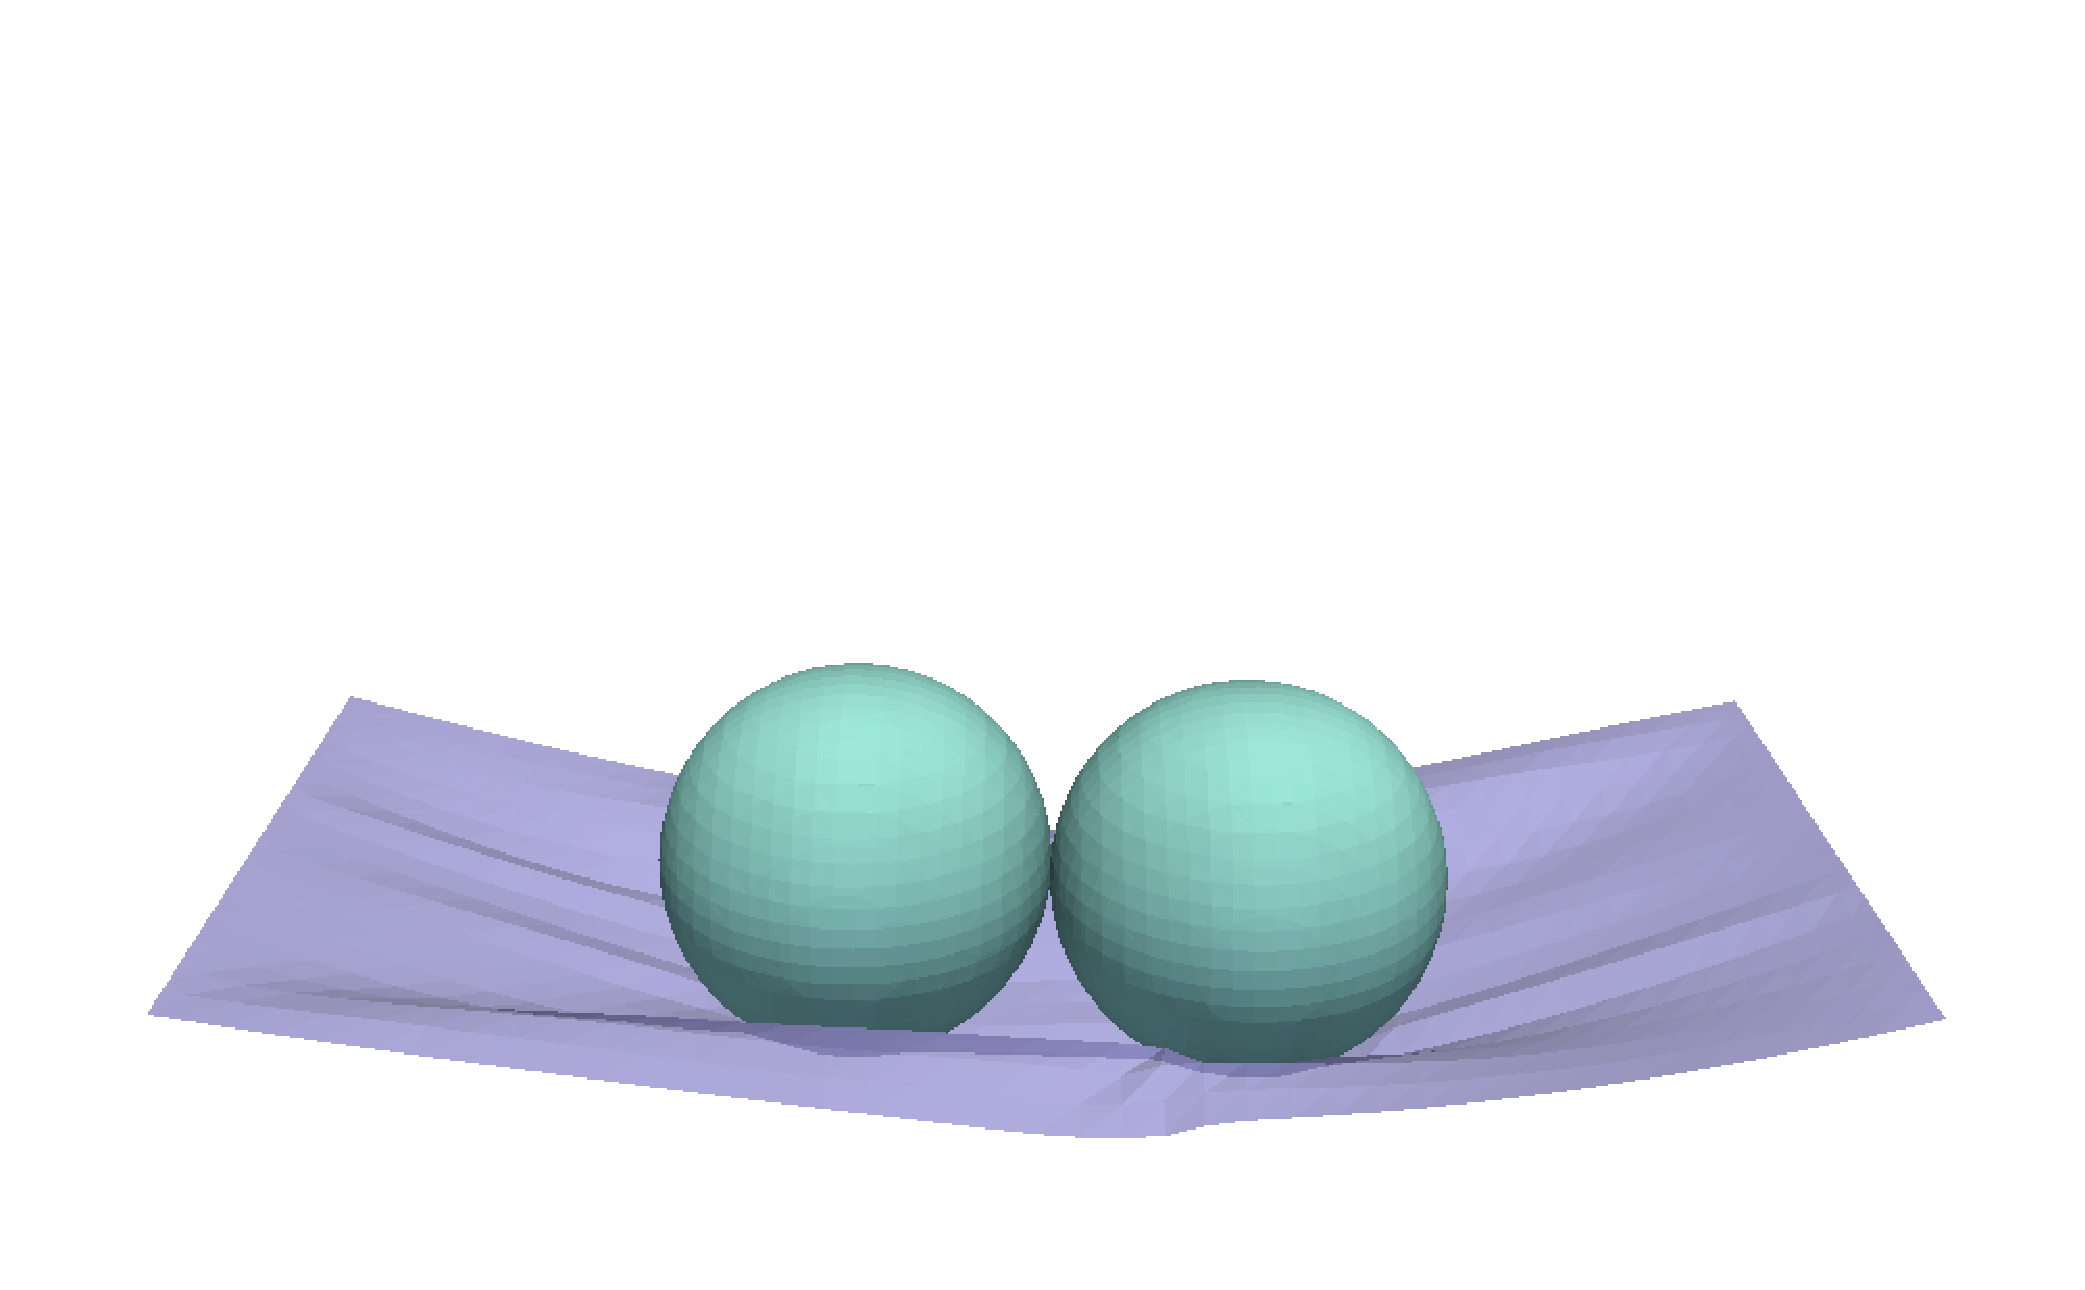
\includegraphics[width=0.48\textwidth]{figures/2sphere_fall_3}
\caption{Two balls falling on to cloth whose two sides are fixed. }
\label{fig:2sphere_fall}
\end{figure}



\newpage
